% Options for packages loaded elsewhere
\PassOptionsToPackage{unicode}{hyperref}
\PassOptionsToPackage{hyphens}{url}
%
\documentclass[
  english,
  ,man,floatsintext]{apa6}
\usepackage{lmodern}
\usepackage{amsmath}
\usepackage{ifxetex,ifluatex}
\ifnum 0\ifxetex 1\fi\ifluatex 1\fi=0 % if pdftex
  \usepackage[T1]{fontenc}
  \usepackage[utf8]{inputenc}
  \usepackage{textcomp} % provide euro and other symbols
  \usepackage{amssymb}
\else % if luatex or xetex
  \usepackage{unicode-math}
  \defaultfontfeatures{Scale=MatchLowercase}
  \defaultfontfeatures[\rmfamily]{Ligatures=TeX,Scale=1}
\fi
% Use upquote if available, for straight quotes in verbatim environments
\IfFileExists{upquote.sty}{\usepackage{upquote}}{}
\IfFileExists{microtype.sty}{% use microtype if available
  \usepackage[]{microtype}
  \UseMicrotypeSet[protrusion]{basicmath} % disable protrusion for tt fonts
}{}
\makeatletter
\@ifundefined{KOMAClassName}{% if non-KOMA class
  \IfFileExists{parskip.sty}{%
    \usepackage{parskip}
  }{% else
    \setlength{\parindent}{0pt}
    \setlength{\parskip}{6pt plus 2pt minus 1pt}}
}{% if KOMA class
  \KOMAoptions{parskip=half}}
\makeatother
\usepackage{xcolor}
\IfFileExists{xurl.sty}{\usepackage{xurl}}{} % add URL line breaks if available
\IfFileExists{bookmark.sty}{\usepackage{bookmark}}{\usepackage{hyperref}}
\hypersetup{
  pdftitle={Are translation equivalents special? Evidence from simulations and empirical data from bilingual infants},
  pdfauthor={Rachel Ka-Ying Tsui1, Ana Maria Gonzalez-Barrero1, Esther Schott1, \& Krista Byers-Heinlein1},
  pdflang={en-EN},
  pdfkeywords={bilingualism, infants, translation equivalents, vocabulary development, word learning, computational modeling},
  hidelinks,
  pdfcreator={LaTeX via pandoc}}
\urlstyle{same} % disable monospaced font for URLs
\usepackage{graphicx}
\makeatletter
\def\maxwidth{\ifdim\Gin@nat@width>\linewidth\linewidth\else\Gin@nat@width\fi}
\def\maxheight{\ifdim\Gin@nat@height>\textheight\textheight\else\Gin@nat@height\fi}
\makeatother
% Scale images if necessary, so that they will not overflow the page
% margins by default, and it is still possible to overwrite the defaults
% using explicit options in \includegraphics[width, height, ...]{}
\setkeys{Gin}{width=\maxwidth,height=\maxheight,keepaspectratio}
% Set default figure placement to htbp
\makeatletter
\def\fps@figure{htbp}
\makeatother
\setlength{\emergencystretch}{3em} % prevent overfull lines
\providecommand{\tightlist}{%
  \setlength{\itemsep}{0pt}\setlength{\parskip}{0pt}}
\setcounter{secnumdepth}{-\maxdimen} % remove section numbering
% Make \paragraph and \subparagraph free-standing
\ifx\paragraph\undefined\else
  \let\oldparagraph\paragraph
  \renewcommand{\paragraph}[1]{\oldparagraph{#1}\mbox{}}
\fi
\ifx\subparagraph\undefined\else
  \let\oldsubparagraph\subparagraph
  \renewcommand{\subparagraph}[1]{\oldsubparagraph{#1}\mbox{}}
\fi
% Manuscript styling
\usepackage{upgreek}
\captionsetup{font=singlespacing,justification=justified}

% Table formatting
\usepackage{longtable}
\usepackage{lscape}
% \usepackage[counterclockwise]{rotating}   % Landscape page setup for large tables
\usepackage{multirow}		% Table styling
\usepackage{tabularx}		% Control Column width
\usepackage[flushleft]{threeparttable}	% Allows for three part tables with a specified notes section
\usepackage{threeparttablex}            % Lets threeparttable work with longtable

% Create new environments so endfloat can handle them
% \newenvironment{ltable}
%   {\begin{landscape}\centering\begin{threeparttable}}
%   {\end{threeparttable}\end{landscape}}
\newenvironment{lltable}{\begin{landscape}\centering\begin{ThreePartTable}}{\end{ThreePartTable}\end{landscape}}

% Enables adjusting longtable caption width to table width
% Solution found at http://golatex.de/longtable-mit-caption-so-breit-wie-die-tabelle-t15767.html
\makeatletter
\newcommand\LastLTentrywidth{1em}
\newlength\longtablewidth
\setlength{\longtablewidth}{1in}
\newcommand{\getlongtablewidth}{\begingroup \ifcsname LT@\roman{LT@tables}\endcsname \global\longtablewidth=0pt \renewcommand{\LT@entry}[2]{\global\advance\longtablewidth by ##2\relax\gdef\LastLTentrywidth{##2}}\@nameuse{LT@\roman{LT@tables}} \fi \endgroup}

% \setlength{\parindent}{0.5in}
% \setlength{\parskip}{0pt plus 0pt minus 0pt}

% \usepackage{etoolbox}
\makeatletter
\patchcmd{\HyOrg@maketitle}
  {\section{\normalfont\normalsize\abstractname}}
  {\section*{\normalfont\normalsize\abstractname}}
  {}{\typeout{Failed to patch abstract.}}
\patchcmd{\HyOrg@maketitle}
  {\section{\protect\normalfont{\@title}}}
  {\section*{\protect\normalfont{\@title}}}
  {}{\typeout{Failed to patch title.}}
\makeatother
\shorttitle{Are translation equivalents special for bilingual infants?}
\keywords{bilingualism, infants, translation equivalents, vocabulary development, word learning, computational modeling}
\usepackage{lineno}

\linenumbers
\usepackage{csquotes}
\usepackage{amsmath}
\usepackage[labelformat=empty]{caption}
\usepackage{caption}
\renewcommand{\topfraction}{1}
\renewcommand{\bottomfraction}{1}
\renewcommand{\textfraction}{.1}
\renewcommand{\floatpagefraction}{1}
\setcounter{topnumber}{9}
\setcounter{bottomnumber}{9}
\setcounter{totalnumber}{20}
\setcounter{dbltopnumber}{9}
\DeclareUnicodeCharacter{2265}{\ensuremath{\ge}}
\DeclareUnicodeCharacter{2264}{\ensuremath{\le}}
\ifxetex
  % Load polyglossia as late as possible: uses bidi with RTL langages (e.g. Hebrew, Arabic)
  \usepackage{polyglossia}
  \setmainlanguage[]{english}
\else
  \usepackage[shorthands=off,main=english]{babel}
\fi
\ifluatex
  \usepackage{selnolig}  % disable illegal ligatures
\fi
\newlength{\cslhangindent}
\setlength{\cslhangindent}{1.5em}
\newlength{\csllabelwidth}
\setlength{\csllabelwidth}{3em}
\newenvironment{CSLReferences}[2] % #1 hanging-ident, #2 entry spacing
 {% don't indent paragraphs
  \setlength{\parindent}{0pt}
  % turn on hanging indent if param 1 is 1
  \ifodd #1 \everypar{\setlength{\hangindent}{\cslhangindent}}\ignorespaces\fi
  % set entry spacing
  \ifnum #2 > 0
  \setlength{\parskip}{#2\baselineskip}
  \fi
 }%
 {}
\usepackage{calc}
\newcommand{\CSLBlock}[1]{#1\hfill\break}
\newcommand{\CSLLeftMargin}[1]{\parbox[t]{\csllabelwidth}{#1}}
\newcommand{\CSLRightInline}[1]{\parbox[t]{\linewidth - \csllabelwidth}{#1}\break}
\newcommand{\CSLIndent}[1]{\hspace{\cslhangindent}#1}

\title{Are translation equivalents special? Evidence from simulations and empirical data from bilingual infants}
\author{Rachel Ka-Ying Tsui\textsuperscript{1}, Ana Maria Gonzalez-Barrero\textsuperscript{1}, Esther Schott\textsuperscript{1}, \& Krista Byers-Heinlein\textsuperscript{1}}
\date{}


\affiliation{\vspace{0.5cm}\textsuperscript{1} Concordia University}

\abstract{
The acquisition of translation equivalents is often considered a special component of bilingual children's vocabulary development, as bilinguals have to learn words that share the same meaning across their two languages. This study examined three contrasting accounts for bilingual children's acquisition of translation equivalents relative to words that are first labels for a referent: the Avoidance Account whereby translation equivalents are harder to learn, the Preference Account whereby translation equivalents are easier to learn, and the Neutral Account whereby translation equivalents are similar to learn. To adjudicate between these accounts, Study 1 explored patterns of translation equivalent learning under a novel computational model --- the Bilingual Vocabulary Model --- which quantifies translation equivalent knowledge as a function of the probability of learning words in each language, and includes a bias parameter that varies the difficulty of learning translation equivalents according to each account. Study 2 tested model-derived predictions against vocabulary data from 200 French--English bilingual children aged 18--33 months. Results showed a close match between the model predictions and bilingual children's patterns of translation equivalent learning. At smaller vocabulary sizes, data matched the Preference Account, while at larger vocabulary sizes they matched the Neutral Account. Our findings show that patterns of translation equivalent learning emerge predictably from the word learning process, and potentially reveal a qualitative shift in translation equivalent learning as bilingual children develop and learn more words.
}



\begin{document}
\maketitle

\captionsetup[table]{labelformat=empty}

Bilingual children must learn words that take a different form in each of their languages, but share the same or highly similar meanings. For instance, to refer to the same crisp red-skinned fruit, an English--French bilingual child must use the word ``apple'' when speaking English, and the word \emph{``pomme''} when speaking French. These cross-language synonyms are known as translation equivalents (also called doublets; Umbel et al., 1992), and are observed amongst bilingual children's first words (e.g., David \& Wei, 2008; De Houwer et al., 2006; Pearson et al., 1995). Translation equivalents are thought to hold a special status in a bilingual's developing lexicon due to the strong overlap in their semantics. For example, studies with bilingual toddlers show that the associative semantic properties of a word in one language facilitate the activation of its translation equivalent (e.g., Bilson et al., 2015; Floccia et al., 2020; Jardak \& Byers-Heinlein, 2019). That is, upon hearing the English word ``apple,'' the corresponding French word \emph{``pomme''} is more easily activated in bilinguals' minds. In vocabulary acquisition, bilingual children must learn a first label for a referent (a ``singlet''; Umbel et al., 1992) before they can learn its translation equivalent (i.e., a second label for a referent learned following a singlet)\footnote{We note that in some cases a singlet may not have a close translation equivalent, for example the recently popular Danish word \emph{``hygge''} refers to a type of cozy contentment and enjoyment of simplicity. Moreover, even when a word that could be considered a translation equivalent exists, adults' concepts may not be congruent across languages (e.g., Malt \& Majid, 2013). However, in early development, vocabulary words tend to be concrete, and evidence suggests that concepts are largely shared across languages (Storm et al., 2020; White et al., 2020). Thus, we make the assumption that most early words have a translation equivalent and that these are fairly congruent for the age range of focus in the current paper.}. Is translation equivalent learning different from singlet learning? The current paper contrasts three competing accounts: 1) translation equivalents are harder to learn than singlets (Avoidance Account), 2) translation equivalents are easier to learn than singlets (Preference Account), and 3) translation equivalents are similar to learn as singlets (Neutral Account). To adjudicate between these accounts, we introduce the Bilingual Vocabulary Model, which provides a computational account of vocabulary learning, with parameters including bilinguals' vocabulary in each language and their developmental level. In Study 1, we use the Bilingual Vocabulary Model to derive a set of predictions, which we then test against vocabulary data from 200 18- to 33-month-old bilingual children in Study 2.

\hypertarget{accounts-of-translation-equivalent-learning}{%
\subsection{Accounts of translation equivalent learning}\label{accounts-of-translation-equivalent-learning}}

\hypertarget{avoidance-account-translation-equivalents-are-harder-to-learn-than-singlets}{%
\subsubsection{Avoidance Account: Translation equivalents are harder to learn than singlets}\label{avoidance-account-translation-equivalents-are-harder-to-learn-than-singlets}}

Early theories of bilingual development claimed that translation equivalents are conspicuously missing from bilingual children's early vocabularies (e.g., Imedadze, 1967; Swain \& Wesche, 1975; Volterra \& Taeschner, 1978). The phenomenon of missing translation equivalents led theorists to propose that young bilingual children do not differentiate their languages, and thus tend to learn only a single word for each referent. This avoidance of translation equivalents --- particularly for nouns --- was thought to be due to word learning biases such as mutual exclusivity, whereby children assume that a referent is only associated with one word at the basic level (Markman, 1992, 1994; Markman \& Wachtel, 1988). For example, when monolingual children see a familiar object (e.g., a cup) next to a novel object (e.g., a garlic press) and hear a novel word like ``wug,'' they assume that ``wug'' refers to the garlic press --- the object unknown to them --- rather than to the cup, the object for which they already know the word.

Although mutual exclusivity is helpful for monolingual vocabulary acquisition, its use is more complex for bilingual vocabulary acquisition (Byers-Heinlein \& Werker, 2009; Davidson \& Tell, 2005; Houston-Price et al., 2010). When encountering a potential singlet, mutual exclusivity would be equally useful for bilinguals as it is for monolinguals, supporting them in associating an unlabeled referent with a novel word. However, a strong form of mutual exclusivity might prevent bilinguals from associating a translation equivalent word with its referent, given that in this case the referent is already associated with another word (albeit in the other language). Thus, mutual exclusivity could prevent bilinguals from acquiring translation equivalents, leading to an abundance of singlets in their vocabularies.

Contrary to earlier studies, more recent work has indicated that bilinguals do understand and produce translation equivalents from early in development (David \& Wei, 2008; De Houwer et al., 2006; Holowka et al., 2002; Legacy et al., 2017; Pearson et al., 1995). Indeed, experimental work has suggested bilingual experience in infancy might not support the development of one-to-one mapping biases such as mutual exclusivity, at least in early infancy. For example, when hearing a novel word like ``nil,'' monolingual children aged 17--22 months looked towards a novel object rather than a familiar object, but bi- and multilingual children looked similarly to both objects (Byers-Heinlein \& Werker, 2009; 2013; Houston-Price et al., 2010). A recent meta-analysis also indicated that bilingual children show mutual exclusivity to a weaker degree than monolinguals (Lewis et al., 2020).

Overall, converging evidence refutes the position that a strong form of mutual exclusivity prevents bilinguals from acquiring translation equivalents. Nonetheless, it leaves open the possibility that translation equivalents may be less likely acquired in favour of learning singlets even if translation equivalents are not completely avoided. If bilingual children avoid lexical overlap across languages even to a small degree, then under the Avoidance Account translation equivalents would be harder to learn than singlets.

\hypertarget{preference-account-translation-equivalents-are-easier-to-learn-than-singlets}{%
\subsubsection{Preference Account: Translation equivalents are easier to learn than singlets}\label{preference-account-translation-equivalents-are-easier-to-learn-than-singlets}}

Contrary to the Avoidance Account, the Preference Account posits that translation equivalents are easier to learn than singlets. At a minimum, word learning requires encoding and representing the relevant sounds of a word, creating a mental representation of its referent, and linking the two. When a French--English bilingual child encounters the word \emph{``pomme''} after having learned ``apple,'' one part of that process has already occurred in that the referent is already represented; because part of the word learning task is already accomplished, translation equivalents might therefore be easier to learn than singlets (e.g., Montanari, 2010; Poulin-Dubois et al., 2013; 2018). Moreover, research suggests that bilingual lexicons are not tightly encapsulated by language, but instead include cross-language mental links between words that are semantically related (e.g., Floccia et al., 2020; Jardak \& Byers-Heinlein, 2019; Singh, 2014). In this context, the strong semantic overlap makes translation equivalents special, and could facilitate their acquisition (e.g., Bilson et al., 2015; Floccia et al., 2020). The Preference Account predicts that translation equivalents are more easily learned than singlets.

There are several lines of empirical evidence to support the Preference Account. For example, some early case studies reported that bilinguals tended to learn more translation equivalents than singlets when experiencing a shift in their language exposure that inverted their dominant and non-dominant languages (Lanvers, 1999; Pearson \& Fernández, 1994). The main explanation that has been given for this finding is that additional exposure to their non-dominant language --- which became their new dominant language --- enabled fast mapping of words to already-lexicalized concepts.

Other evidence suggesting translation equivalents might be easier to learn than singlets comes from a study that included vocabulary-checklist data from 254 monolingual and 181 bilingual children aged 6 months to 7.5 years (Bilson et al., 2015). The researchers used a network analysis approach to investigate how translation equivalents are learned, focusing on the semantic relationships between the words (e.g., words like ``cat'' and ``dog'' are strongly semantically related). Using a statistical model that allowed free semantic relations among vocabulary data from monolingual and bilingual children, the results suggested that words were learned faster when they were semantically connected to more known words in children's lexicons. This effect applied not only to words within the same language, but also to words across languages including translation equivalents (e.g., English ``dog'' and French \emph{``chien''}) and words that had other cross-language relations (e.g., ``cat'' and \emph{``chien''}). The authors then simulated bilingual vocabulaires by modeling bilingual lexicons as combinations of two independent vocabulary-size-matched monolinguals. Comparison with actual bilingual children's vocabulary data revealed that bilingual children acquired more translation equivalents than predicted by the simulation. The authors therefore concluded that bilingual children learn translation equivalents more easily than singlets. Note that, in their study, expected translation equivalent knowledge was simulated based on the number of lexical items that overlapped between two randomly chosen English monolinguals (e.g., whether both monolinguals knew the word ``cat''). However, it is unclear whether this is an appropriate point of comparison for bilingual children as this approach may overlook variables that impact bilinguals' vocabulary learning, including vocabulary size in each language and the developmental level of a child --- a point that we will return to later in the introduction.

Overall, there is some evidence that bilingual children more readily learn translation equivalents than singlets. If the strong semantic overlap between translation equivalents facilitates their learning, then under the Preference Account translation equivalents will be more easily learned than singlets.

\hypertarget{neutral-account-translation-equivalents-are-similar-to-learn-as-singlets}{%
\subsubsection{Neutral Account: Translation equivalents are similar to learn as singlets}\label{neutral-account-translation-equivalents-are-similar-to-learn-as-singlets}}

The previous accounts rely on the idea that bilingual vocabulary development unfolds differently than monolingual development, as monolinguals encounter only singlets but bilinguals encounter both singlets and translation equivalents. There is an underlying assumption that translation equivalent learning is somehow special relative to singlet learning --- the Avoidance Account proposes that translation equivalents are harder to learn than singlets, whereas the Preference Account proposes that translation equivalents are easier to learn than singlets. However, it is also possible that translation equivalents are neither harder nor easier for bilingual children to learn than singlets. We call this the Neutral Account.

The Neutral Account implies that bilingual children's two languages develop relatively independently. Indeed, language and processing measures for bilingual children tend to be tightly correlated within a particular language, and weakly if at all correlated across languages. For example, 30-month-old bilingual children's processing efficiency in a particular language closely correlated with vocabulary size in that language, but was unrelated to vocabulary size in their other language (Marchman et al., 2010). Due to differences in the amount of language exposure, bilingual children seldom show equal vocabulary growth in both of their languages (e.g., Pearson \& Fernandez, 1994; Pearson et al., 1997), and the amount of exposure to a particular language has been reported to modulate the within-language association between language processing ability and vocabulary size (Hurtado et al., 2014). Bilingual children with greater exposure to a particular language tended to process that language faster, and in turn learned more words in that language.

In a study whose results support the Neutral Account, Pearson and colleagues (1995) randomly paired the single-language English lexicons from a subset of bilingual children to the single-language Spanish lexicons from another subset of bilingual children to derive a percentage of by-chance lexical overlaps shared between monolingual lexicons of two randomly paired children. The researchers found that the percentage of translation equivalents observed in English--Spanish bilingual children was similar to the by-chance percentage of translation equivalents between randomly-paired children. This evidence implied that singlets and translation equivalents are equally learnable, although the paper was limited by its somewhat small sample (\emph{n} = 27) in the context of a wide age range (8 months to 2.5 years). In sum, the Neutral Account predicts that translation equivalents are similar for bilingual children to learn as singlets.

\hypertarget{contributors-to-translation-equivalent-knowledge}{%
\subsection{Contributors to translation equivalent knowledge}\label{contributors-to-translation-equivalent-knowledge}}

The previous section discussed three theoretical accounts concerning the relative learnability of translation equivalents. However, to date, aspects of translation equivalent learning have mostly been examined in isolation, rather than integrated within the larger context of bilingual lexical development. In this section, we consider two proximal variables that we expect to predict the number of translation equivalents bilingual children know: vocabulary size in each language, and word learnability as a function of children's developmental level.

\hypertarget{vocabulary-size-in-bilinguals-two-languages}{%
\subsubsection{Vocabulary size in bilinguals' two languages}\label{vocabulary-size-in-bilinguals-two-languages}}

Balance between the two vocabulary sizes is a function of the number of words bilingual children produce in each language, which tends to be tightly linked to their exposure to each language. In general, more language exposure leads to larger vocabulary size (e.g., Barnes \& Garcia, 2013; Boyce et al., 2013; Hurtado et al., 2014; Marchman et al., 2010; Pearson et al., 1997; Place \& Hoff, 2011). Bilingual children usually know more words in the language in which they have greater exposure (i.e; dominant language) relative to the language in which they have less exposure (i.e., non-dominant language; Pearson et al., 1997; Place \& Hoff, 2011). This is because the more often a bilingual hears a language, the more opportunities there will be for learning new words in that language.

Because translation equivalents are words from different languages that refer to the same concept, the number of words a bilingual knows in each of their languages will necessarily constrain the number of translation equivalent pairs they could possibly know. For example, a child with a less balanced vocabulary across the two languages might only say 5 words in one language but many more words in the other language; this means that the child could only produce a maximum of 5 translation equivalents, regardless of how many words they know in their other language. Conversely, it seems reasonable to expect that if a child knows a similar number of words in each language and thus has a more balanced vocabulary across the two languages, there would be more potential for some of those words to be translation equivalents.

\hypertarget{word-learnability-as-a-function-of-developmental-level}{%
\subsubsection{Word learnability as a function of developmental level}\label{word-learnability-as-a-function-of-developmental-level}}

An often overlooked factor that could contribute to bilingual children's learning of translation equivalents is related to the changes in the learnability of different words over time based on children's developmental level. Evidence from monolingual children shows that some types of words are characteristically learned before others. For example, across many languages including English, children show a noun bias in their early lexicons (Braginsky et al., 2019; Goodman et al., 2008), although for other languages such as Mandarin it appears that verbs and nouns are more equally acquired (Tardif, 1996). Certain classes of words are rarely known at the onset of lexical development, such as prepositions and words for time (Fenson et al., 2007). This is thought to be due to the cognitive and linguistic machinery that must be in place in order for children to represent these concepts, a necessary prerequisite for learning certain word types (Bergelson, 2020; Braginsky et al., 2019). If this is the case, then children might be more likely to learn translation equivalents than singlets, simply because translation equivalents are more likely to be learnable at their stage of development. That is, many potential singlets could be ``too hard'' to be learned at a particular age, while by definition potential translational equivalents refer to concepts that children are already able to lexicalize. For example, an 14-month-old who has learned the French words \emph{``ballon''} and \emph{``chien''} would be capable of learning their translation equivalents ``ball'' and ``dog,'' as easier potential singlets like ``cup,'' but not later-acquired potential singlets like ``tomorrow,'' ``who,'' or ``not.'' Thus, a seeming overabundance of translation equivalents might be a product of developmental constraints on word learning, rather than due to semantic facilitation.

\hypertarget{the-bilingual-vocabulary-model}{%
\subsection{The Bilingual Vocabulary Model}\label{the-bilingual-vocabulary-model}}

Taking into account the contributions of language exposure and developmental level to bilingual children's vocabulary acquisition, we put forward the Bilingual Vocabulary Model. This model proposes that the number of translation equivalents that bilingual children produce is a function of vocabulary learning in each language, in the context of the number of potentially learnable words given the children's developmental level. We formalize learning a translation equivalent pair as the joint probability of learning each of the words in the pair. This provides a straight-forward empirical test of different theoretical accounts of translation equivalent learning, by asking whether or not the probability of knowing a word is independent of knowing its translation equivalent. The logic is similar to that of the familiar chi-squared test for independence, where the independence of two events from the same population is tested as the probability of their intersection computed by multiplying the probability of each individual event: P(A and B) = P(A) × P(B) if A and B are independent\footnote{To test the independence of two events from the same population, as an example, we might ask whether Psychology majors are more likely to be left-handed. Imagine a college of 1000 students. If 100/1000 (or 1/10) students are left-handed, and 200/1000 (or 1/5) students are psychology majors, then if these variables are independent we expect a proportion of 1/10 × 1/5 = 1/50 students to be left-handed psychology majors. To determine the number we expect to observe in the college, we multiply 1/50 × 1000 = 20 students. When we compare this expected number to the actual number of left-handed students, there are three possible outcomes. First, we may observe many more than 20 left-handed psychology students at the college (say 100 students), which suggests that being left-handed increases the probability of majoring in psychology. Or, second, we may observe many fewer than 20 left-handed psychology students at the college (say 5 students), which suggests that being left-handed decreases the probability of majoring in psychology (in this example by a factor of 1/4). Finally, if left-handedness and majoring in psychology are independent, we can predict the number of left-handed psychology students by multiplying the observed number of left-handed students (100) by the observed number of psychology students (200), and dividing by the total population of the college (1000), so for example 100×200/1000 = 20. Thus, comparing expected and observed numbers can inform us about the independence of the underlying phenomena.}. In the next paragraphs, we define each of the model parameters in detail, and these are also summarized in Table 1.

The model takes four main parameters: the number of words produced in the dominant language (DOM), the number of words produced in the non-dominant language (NONDOM), vocabulary size of potentially learnable words in each language (LEARNABLE), and a bias parameter (BIAS) which indicates whether the model is biased towards (BIAS \textgreater{} 1) or against (BIAS \textless{} 1) learning translation equivalents. The language in which a child knows more words is the dominant language, whereas the one in which a child knows fewer words is the non-dominant language. Next, we turn to the LEARNABLE parameter (i.e., the number of potentially learnable words). If DOM and NONDOM are measured with an instrument such as the MacArthur-Bates Communicative Development inventories (CDI; Fenson et al., 2007), one option would be to set LEARNABLE to be the total number of items on the CDI. For convenience, consider the effect of setting LEARNABLE to 600, as a round number (the actual number of CDI items is usually slightly higher than 600, depending on the language of the adaptation). However, not all children will be capable of learning all of the CDI words. Typically, words that are more concrete, occur more frequently in the input, and words that are associated with babies tend to be acquired earlier than other words (Braginsky et al., 2019), and very young children would not be expected to produce many of the ``harder'' words on the CDI, such as ``lawn mower,'' ``sidewalk,'' or ``vitamins.'' Thus, a reasonable solution might be to determine how many CDI words are potentially learnable given the child's developmental level, which could be approximated by their age. Since there are no CDI norms for French-English bilingual children, we will take the average English and French CDI norms to approximate how many words children might lexicalize in either language. For example, imagine that Jamie who is 18 months old produces 50 English words and 20 French words, thus a total of 70 words. Monolingual children his age with the very largest productive vocabularies (those at the 90th percentile averaging between English and French norms) produce a total of 240 words (retrieved from the Wordbank database version 0.3.1; Frank et al., 2016). Although there is likely considerable individual variability as to the cognitive capacity even amongst children of the same age, we argue that averaging between the English and French CDIs at the 90th percentile provides a reasonable --- if imperfect --- estimate of the number of learnable words (LEARNABLE) that a bilingual child of Jamie's age could potentially acquire in each language. Thus, we might expect that Jamie could potentially have learned up to 240 words in English and 240 words in French, although he has thus far only learned 50 in English and 20 in French. Note that we model learnability in terms of the number of words expected to be learnable at a particular age, rather than modeling the learnability of individual words at a particular age --- a simplifying choice that we will return to in the discussion section.

Using the mathematical concept of independence, we can then quantify the number of translation equivalents (TE) expected given children's vocabulary sizes in the dominant (DOM) and non-dominant (NONDOM) languages, as well as the number of potentially learnable words (LEARNABLE). If dominant-language and non-dominant-language words are learned independently from each other, we multiply DOM × NONDOM (the number of words known in the dominant and non-dominant language respectively), and divide by the total population of learnable words in one language (LEARNABLE) --- which is the possible number of words that could overlap across both languages --- to predict the number of translation equivalents. We further introduce the bias parameter (BIAS), which allows us to examine whether translation equivalent learning is best described by the Avoidance, Preference, or Neutral Account. Adding this parameter, translation equivalents can be derived from TE = BIAS × (DOM × NONDOM)/LEARNABLE. For the Avoidance Account, BIAS will be less than 1, meaning that translation equivalentsare less easily learned than singlets; for the Preference Account, BIAS will be greater than 1, meaning that translation equivalents are more easily learned than singlets; for the the Neutral Account, BIAS is exactly 1 (i.e., the model is unbiased with respect to whether translation equivalents are more difficult or easier to acquire than singlets). Going back to the example of 18-month-old Jamie, we would set the denominator at 245 which is the number of potentially learnable words at 18 months. If translation equivalents are half as easy to learn as singlets (following the Avoidance Account), we would expect Jamie to produce .5×(50×20/245) = 2.0 translation equivalents. Conversely, if translation equivalents are twice as easy to learn as singlets (following the Preference Account), we would expect Jamie to produce 2×(50×20/245) = 8.2 translation equivalents. Under the Neutral Account, we would expect Jamie to learn 1×(50×20/245) = 4.1 translation equivalents.

\begin{landscape}\begin{table}

\caption{\label{tab:table1}Table 1. Summary of the parameters in the Bilingual Vocabulary Model.}
\centering
\fontsize{7}{9}\selectfont
\begin{tabular}[t]{l>{\raggedright\arraybackslash}p{175px}>{\raggedright\arraybackslash}p{175px}>{\raggedright\arraybackslash}p{175px}}
\toprule
Variable & Definition & Constraints & Relationship.to.other.parameters\\
\midrule
\addlinespace[0.3em]
\multicolumn{4}{l}{\textbf{Main Parameters}}\\
\hspace{1em}LEARNABLE & Number of learnable words in each language, given the child’s developmental level & Varies by age. No greater than the number of words on CDI. & Maximum number that could be learned in DOM or NONDOM\\
\hspace{1em}DOM & Words produced in the dominant language & DOM ≥ NONDOM (children always produce more words in dominant than non-dominant language); DOM ≤ LEARNABLE & DOM = (1-BALANCE)×WORD; DOM = WORD - NONDOM\\
\hspace{1em}NONDOM & Words produced in the non-dominant language & NONDOM ≤ DOM (children always produce fewer words in non-dominant than dominant language); NONDOM ≤ LEARNABLE & NONDOM = BALANCE×WORD; NONDOM = WORD - DOM\\
\hspace{1em}BIAS & Bias parameter & BIAS < 1 implies the Avoidance Account; BIAS > 1 implies the Preference Account; BIAS = 1 implies the Neutral Account & \\
\addlinespace[0.3em]
\multicolumn{4}{l}{\textbf{Derived Parameters}}\\
\hspace{1em}BALANCE & Balance (relative proportion of words produced in the non-dominant language to the total words produced in both languages) & 0 ≤ BALANCE ≤ .50 (greater values indicate children producing a more similar number of words in their two languages) & BALANCE = NONDOM/WORD; BALANCE = NONDOM/(DOM+NONDOM)\\
\hspace{1em}WORD & Word vocabulary (or total vocabulary size) & W ≤ 2×LEARNABLE (maximum word vocabulary is knowing each word in both languages) & WORD = DOM+NONDOM; WORD = DOM/(1-BALANCE); WORD = NONDOM/(BALANCE)\\
\hspace{1em}TE & Translation equivalents produced &  & TE = BIAS × DOM×NONDOM/LEARNABLE\\
\hspace{1em}CONCEPT & Concept vocabulary (or total conceptual vocabulary size) &  & CONCEPT = WORD - TE; CONCEPT = TE + DOM-SINGLET + NONDOM-SINGLET\\
\hspace{1em}DOM-SINGLET & Singlets in dominant language &  & DOM-SINGLET = DOM - TE\\
\hspace{1em}NONDOM-SINGLET & Singlets in non-dominant language &  & NONDOM\_SINGLET = NONCOM - TE\\
\bottomrule
\multicolumn{4}{l}{\rule{0pt}{1em}\textit{Note: }}\\
\multicolumn{4}{l}{\rule{0pt}{1em}All vocabulary measures are constrained to be integers.}\\
\end{tabular}
\end{table}
\end{landscape}

Finally, based on the main parameters, we can calculate additional, commonly-reported descriptors of bilingual vocabulary, which we detail below and describe as derived parameters.

Balance of vocabulary (BALANCE) is the proportion of total words that children produce in each language. For convenience, balance is defined in reference to the non-dominant language with the formula NONDOM/(DOM+NONDOM), such that scores can range from 0.0 (completely unbalanced) to 0.5 (completely balanced). For example, since 18-month-old Jamie produces 50 dominant vocabulary words and 20 non-dominant vocabulary words, he would have a balance score of 0.29. Note that this calculation does not take into account overlap in meaning across the two languages (i.e., how many of the words he produces are translation equivalents).

Word vocabulary (WORD; sometimes called total productive vocabulary) is the total number of words that a child produces across the two languages, calculated as the sum of the dominant vocabulary (DOM) and non-dominant vocabulary (NONDOM). Concept vocabulary (CONCEPT; sometimes called total conceptual vocabulary) is the number of concepts that are lexicalized by the child --- that is, the total number of concepts that are lexicalized in either language. This can be calculated by subtracting the number of translation equivalents (TE) from the word vocabulary (WORD). Finally, we can also calculate singlets that are produced in each language, that is words for which the child does not yet produce a translation equivalent. Singlets in the dominant language (DOM-SINGLET) can be calculated by subtracting translation equivalents (TE) from dominant-language vocabulary (DOM); singlets in the non-dominant language (NONDOM-SINGLET) can be calculated by subtracting translation equivalents (TE) from non-dominant language vocabulary (NONDOM). It is also possible to decompose children's word vocabulary (WORD) into the sum of TE, DOM-SINGLET, and NONDOM-SINGLET.

Finally, we note two simplifying assumptions made by our model. First, we assume that children have the same communicative need in each language: our model does not account for cases where bilinguals might systematically refer to a concept in only one language and not the other (e.g., Grosjean, 2016). Second, we assume that translation equivalents refer to the same underlying concept. Thus, our model does not consider the nuanced and language-specific conceptual representations that bilingual adults might ultimately develop (Malt \& Majid, 2013; Storm et al., 2015; White et al., 2020). However, we believe that these assumptions present a reasonable first approximation, especially in the case of young children, and return to these assumptions in the discussion section.

\hypertarget{current-studies}{%
\subsection{Current studies}\label{current-studies}}

The current studies aimed to better understand the nature of translation equivalent learning in bilingual children. Study 1 simulated the expected patterns of translation equivalent learning under the Bilingual Vocabulary Model proposed in the introduction, with reference to the proportion of words learned in the dominant and non-dominant language and the number of words that are learnable at various developmental levels. We also compared predicted learning outcomes for when translation equivalents are harder, easier, or similar to learn as singlets.

In Study 2, we examined real-world translation equivalent development in light of the predictions from the Bilingual Vocabulary Model, using archival data from 200 French--English bilingual children aged 18 to 33 months, whose vocabularies and translation equivalent knowledge were measured by parent report using the MacArthur-Bates CDI: Words and Sentences form in English (Fenson et al., 2007) and Québec French (Trudeau et al., 1999). Together, the Bilingual Vocabulary Model and real-world data allowed us to examine contrasting hypotheses about translation equivalents: whether translation equivalents learning is harder (Avoidance Account), easier (Preference Account), or similar (Neutral Account) to learning singlets.

\hypertarget{study-1-simulations}{%
\section{Study 1: Simulations}\label{study-1-simulations}}

Study 1 provides a computational implementation of the Bilingual Vocabulary Model outlined in the introduction, which we use to simulate different scenarios to examine the effect of vocabulary sizes and developmental variables on translation equivalent learning. Note that usually only three values are necessary to calculate all the other variables (see Table 1). Most commonly, we can calculate other variables based on the total number of learnable words (LEARNABLE) together with either the words known in each language (DOM and NONDOM) or word vocabulary plus balance (WORD and BALANCE) which allow us to compute DOM and NONDOM. It is also possible to calculate other variables based on the total number of learnable words (LEARNABLE) with balance and words known in either language (BALANCE and DOM or BALANCE and NONDOM).

We present three simulations generated by creating data points for hypothetical children by varying different parameters of the Bilingual Vocabulary Model, in order to explore expected patterns of translation equivalent learning. The number of children in each simulation was fully determined by the number of levels varied for each parameter: each combination of parameters was included, except for those that violated constraints in the model (e.g., NONDOM could not be larger than DOM). In the first simulation, we examined how translation equivalent learning relates to vocabulary balance (BALANCE), as well as different metrics of vocabulary size, including dominant-language vocabulary (DOM), non-dominant language vocabulary (NONDOM), and word vocabulary (WORD). In the second simulation, we explored relations between translation equivalents (TE), balance (BALANCE), and learnable words (LEARNABLE). In the first two simulations, the BIAS parameter was held constant at 1 (Neutral Account); in the third simulation, we varied the bias parameter (BIAS) to compare translation equivalent learning under the Avoidance, Preference, and Neutral Accounts. A summary of the parameter values used in each simulation is provided in Table 2.

\begin{landscape}\begin{table}

\caption{\label{tab:table2}Table 2. Summary of the parameters used in each simulation.}
\centering
\fontsize{8}{10}\selectfont
\begin{tabular}[t]{>{\centering\arraybackslash}p{45px}>{\raggedright\arraybackslash}p{45px}>{\raggedright\arraybackslash}p{75px}>{\raggedright\arraybackslash}p{75px}>{\raggedright\arraybackslash}p{75px}>{\raggedright\arraybackslash}p{75px}>{\raggedright\arraybackslash}p{75px}>{\raggedright\arraybackslash}p{45px}}
\toprule
Simulation & Learnable words (LEARNABLE) & Words in dominant Language (DOM) & Words in non-dominant language (NONDOM) & Word vocabulary (WORD) & Balance of vocabulary (BALANCE) & Bias parameter (BIAS) & Total number of data points generated\\
\midrule
1 & Constant at 600 & Varied, ranging from 100 to LEARNABLE at an interval of 100 & Varied, ranging from 0 to DOM at an interval of 10 & Calculated as WORD = DOM + NONDOM & Calculated as BALANCE = NONDOM / (DOM+NONDOM) & Constant at 1 & 216\\
2 & Varied at 100, 200, 300, 400, 500, 600 & Varied, ranging from 100 to LEARNABLE at an interval of 100 & Varied, ranging from 0 to DOM at an interval of 20 & Calculated as WORD = DOM + NONDOM & Calculated as BALANCE = NONDOM / (DOM+NONDOM) & Constant at 1 & 301\\
3 & Varied at 150, 300, 450, and 600 & Varied, ranging from 100 to LEARNABLE at an interval of 100 & Varied, ranging from 0 to DOM at an interval of 25 & Calculated as WORD = DOM + NONDOM & Calculated as BALANCE = NONDOM / (DOM+NONDOM) & Varied at 0.5 (Avoidance Account), 1 (Neutral Account), and 1.5 (Preference Account) & 166\\
\bottomrule
\end{tabular}
\end{table}
\end{landscape}

\hypertarget{simulation-1-children-of-the-same-developmental-level-with-different-word-vocabularies-and-balances-of-vocabulary}{%
\subsection{1.1 Simulation 1: Children of the same developmental level with different word vocabularies and balances of vocabulary}\label{simulation-1-children-of-the-same-developmental-level-with-different-word-vocabularies-and-balances-of-vocabulary}}

In Simulation 1, we first illustrate the relationships between different variables in the model by simulating three hypothetical children who are at the same developmental level and thus have the same number of potentially learnable words (LEARNABLE), but with different word vocabularies (WORD) and BALANCE. For convenience, we set LEARNABLE = 600 in this example, which roughly corresponds to what is expected for an English-French 27-month-old bilingual child (i.e., the most verbal 27-month-old English-learner at the 90th percentile of vocabulary produces around 633 words and the most verbal 27-month-old French-learner produces around 580 words as retrieved from the Wordbank database, giving us an average of 606 words across the two languages; Frank et al., 2016). We set BIAS to 1, meaning that in these examples translation equivalents are equally easy to learn as singlets.

We first illustrate with three simulated children. Infant Annie (small vocabulary, unbalanced exposure) produces 270 words in the dominant language and 30 words in her non-dominant language. She has a word vocabulary of 300, and a balance score of .10 (10\% of her words are in the non-dominant language). Based on the formula TE = DOM×NONDOM/LEARNABLE (we drop BIAS from the formula since it is 1 here) and as seen in Table 3, Annie is expected to produce 13.5 translation equivalents. Infant Bernie (small vocabulary, balanced exposure) produces 180 dominant-language words, and 120 non-dominant language words. Like Annie, he has a word vocabulary of 300, but he has a higher balance score of .40 (40\% of his words are in the non-dominant language). Based on our formula, we expect Bernie to produce 36 translation equivalents. Comparing Annie and Bernie, two children who produce the same word vocabulary (i.e., WORD is held constant), the child with more balanced language vocabulary (Bernie) is expected to produce more translation equivalents. Like Bernie, infant Charlie also has a balanced vocabulary, but has a larger word vocabulary (WORD), producing 540 words in the dominant language (DOM) and 360 in the non-dominant language (NONDOM) for a total of 900 words (WORD), and thus BALANCE = .40. Based on our formula for Simulation 1, we expect Charlie to produce 324 translation equivalents (TE). Infants Bernie and Charlie illustrate that for two children equal in BALANCE, the child with larger word vocabulary (WORD) is expected to produce more translation equivalents (TE). Other vocabulary metrics are calculated for each hypothetical child as described in Table 3.

We then broadened this simulation to the more general case and examined patterns of translation equivalent learning, where simulated children had the capacity to learn 600 words (LEARNABLE held constant at 600), and their vocabulary size in each language (DOM and NONDOM) varied. BIAS was once again constant at 1. Data from a total of 216 simulated children were generated (see Table 2 for a summary of the parameter values used in this simulation). Based on these values, we derived simulated children's word vocabulary (WORD, calculated as DOM+NONDOM) and their vocabulary balance (BALANCE, calculated as NONDOM/(DOM+NONDOM)). In Figure 1, we plotted TE knowledge as a function of DOM, NONDOM, and WORD at different levels of BALANCE. Across all three Panels (1A, 1B, and 1C), simulated children with the most balanced vocabulary consistently produced more translation equivalents than other children. Moreover, Panels 1A and 1C show that, as the number of DOM (dominant language words) and WORD (word vocabulary) increased, TE also increased regardless of BALANCE. Interestingly, Panel 1B shows that NONDOM and TE were extremely tightly coupled. In sum, we observed three important patterns, which served as Prediction Set 1 from the Bilingual Vocabulary Model for Study 2:

\begin{landscape}\begin{table}

\caption{\label{tab:table3}Table 3. Examples for Simulation 1 of three hypothetical children with different hypothetical word vocabularies (WORD) and vocabulary balance (BALANCE), where the number of learnable words (LEARNABLE) = 600 and BIAS = 1. Vocabulary values are rounded to the nearest integer.}
\centering
\fontsize{8}{10}\selectfont
\begin{tabular}[t]{>{\raggedright\arraybackslash}p{100px}>{\raggedright\arraybackslash}p{140px}>{\raggedright\arraybackslash}p{140px}>{\raggedright\arraybackslash}p{60px}>{\raggedright\arraybackslash}p{60px}>{\raggedright\arraybackslash}p{60px}}
\toprule
Variable & Definition & Calculation & Infant Anne (small vocabulary, unbalanced) & Infant Bernie (small vocabulary, balanced) & Infant Charlie (large vocabulary, balanced)\\
\midrule
\addlinespace[0.3em]
\multicolumn{6}{l}{\textbf{Main Parameters}}\\
\hspace{1em}BIAS & Bias parameter &  & 1 & 1 & 1\\
\hspace{1em}LEARNABLE & Learnable words in each language &  & 600 & 600 & 600\\
\hspace{1em}DOM & Words produced in the dominant language &  & 270 & 180 & 540\\
\hspace{1em}NONDOM & Words produced in the non-dominant language &  & 30 & 120 & 360\\
\addlinespace[0.3em]
\multicolumn{6}{l}{\textbf{Derived Parameters}}\\
\hspace{1em}WORD & Word vocabulary (or total vocabulary size) & DOM + NONDOM & 300 & 300 & 900\\
\hspace{1em}BALANCE & Vocabulary balance & NONDOM / (DOM + NONDOM) & 0 & 0 & 0\\
\hspace{1em}TE & Translation equivalents produced & DOM × NONDOM / LEARNABLE & 14 & 36 & 324\\
\hspace{1em}CONCEPT & Concept vocabulary (or total conceptual vocabulary size) & WORD - TE & 286 & 264 & 576\\
\hspace{1em}DOM-SINGLET & Singlets in dominant language & DOM - TE & 256 & 144 & 216\\
\hspace{1em}NONDOM-SINGLET & Singlets in non-dominant language & NONDOM - TE & 16 & 84 & 36\\
\bottomrule
\end{tabular}
\end{table}
\end{landscape}

\begin{itemize}
\tightlist
\item
  Prediction 1a: Children with more balanced vocabularies (BALANCE) will produce more translation equivalents (TE) (Figure 1, Panel 1A).
\item
  Prediction 1b: Children who produce more total words (WORD) or more dominant-language words (DOM) will produce more translation equivalents (TE) (Figure 1, Panels 1A and 1B).
\item
  Prediction 1c: Children who produce more non-dominant language words (NONDOM) will produce more translation equivalents (TE). Unlike for WORD and DOM this will not interact with BALANCE; instead, non-dominant vocabulary size will be an almost perfect predictor of translation equivalent knowledge (Figure 1, Panel 1C).
\end{itemize}

\begin{figure}[H]

{\centering 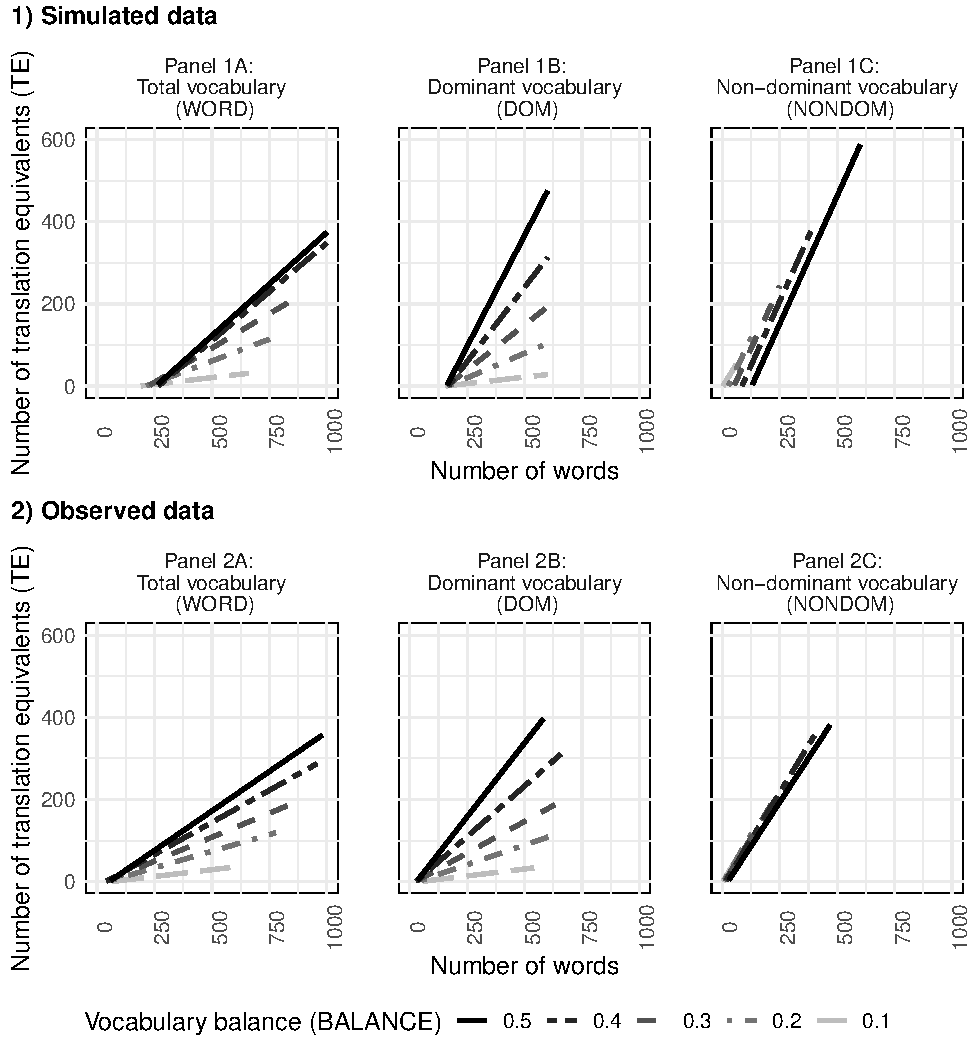
\includegraphics[width=1.1\linewidth,height=0.8\textheight]{paper_TE_bilingual_vocabulary_model_files/figure-latex/fig1-1} 

}

\caption{Number of translation equivalents (TE) across different levels of vocabulary balance (BALANCE) in relation to word vocabulary (WORD; Panel A), dominant vocabulary size (DOM; Panel B), and non-dominant vocabulary size (NONDOM; Panel C). Row 1 plots the simulated data in Study 1 while holding the number of learnable words (LEARNABLE) constant at 600 and BIAS constant at 1. Row 2 plots the observed vocabulary data in Study 2.}\label{fig:fig1}
\end{figure}

\hypertarget{simulation-2-acquisition-of-translation-equivalents-and-singlets-at-different-developmental-levels}{%
\subsection{1.2 Simulation 2: Acquisition of translation equivalents and singlets at different developmental levels}\label{simulation-2-acquisition-of-translation-equivalents-and-singlets-at-different-developmental-levels}}

In our previous simulation, we assumed that each simulated child was at the same developmental level and had the capacity to learn up to 600 words in each language (i.e., LEARNABLE held constant at 600). As laid out in the introduction, under the Bilingual Vocabulary Model, the learnability of different words changes with a child's developmental level, where LEARNABLE increases as a child grows older. Therefore, in Simulation 2, we looked at the expected patterns of translation equivalent learning across varying levels of LEARNABLE (i.e., the number of learnable words in each language as developmental level changes). Additionally, we further examined vocabulary composition by computing the number of singlets in the dominant (DOM-SINGLET) and non-dominant (NONDOM-SINGLET) language. BIAS was once again kept constant at 1.

Translation equivalent knowledge was simulated across children at six developmental levels (the number of LEARNABLE words = 100, 200, 300, 400, 500, 600), in conjunction with a wide range of values for words in the dominant language (DOM) and the non-dominant language (NONDOM). In total, data from 301 simulated children were generated (see Table 2 for a summary of the parameters used in this simulation). Again, balance (BALANCE) was calculated based on the values of DOM and NONDOM. We also calculated the number of singlet words in the dominant (DOM-SINGLET) and non-dominant (NONDOM-SINGLET) languages by the formula DOM-SINGLET = DOM - TE and NONDOM-SINGLET = NONDOM - TE. Figure 2 plots the number of CONCEPT, TE, DOM-SINGLET, and NONDOM-SINGLET at different BALANCE levels across different levels of LEARNABLE. As shown in Panel 1A, simulated children at a later developmental level had larger concept vocabularies (CONCEPT). In Panel 1B, we continued to observe a pattern reported in prediction 1a, whereby simulated children with more balanced vocabularies produced more translation equivalents (TE). Moreover, regardless of balance, simulated children at later developmental levels (i.e., older children with more potentially LEARNABLE words) acquired more translation equivalents (TE). Panels 1C and 1D show that simulated children at later developmental levels also produced more singlets in the dominant and non-dominant languages, and that more balanced children would produce more singlets in their non-dominant language, but fewer singlets in their dominant language than less balanced children. Overall, we generated 4 additional predictions (Prediction Set 2) made by the Bilingual Vocabulary Model. Compared to children at an earlier developmental level (i.e., younger infants with fewer potentially learnable words), children at a later developmental level (i.e., older infants with more potentially learnable words) will

\begin{itemize}
\tightlist
\item
  Prediction 2a: Have larger concept vocabularies (CONCEPT). (Figure 2, Panel 1A)
\item
  Prediction 2b: Produce more translation equivalents (TE), regardless of vocabulary balance (BALANCE). (Figure 2, Panel 1B)
\item
  Prediction 2c: Produce more dominant-language singlet words (DOM-SINGLET). Moreover, those with the least \emph{balanced} vocabulary (BALANCE) will produce the most DOM-SINGLET. (Figure 2, Panel 1C)
\item
  Prediction 2d: Produce more non-dominant-language singlets (NONDOM-SINGLET). Moreover, those with the most \emph{balanced} vocabulary (BALANCE) will produce the most NONDOM-SINGLET. (Figure 2, Panel 1D)
\end{itemize}

\begin{figure}[H]

{\centering 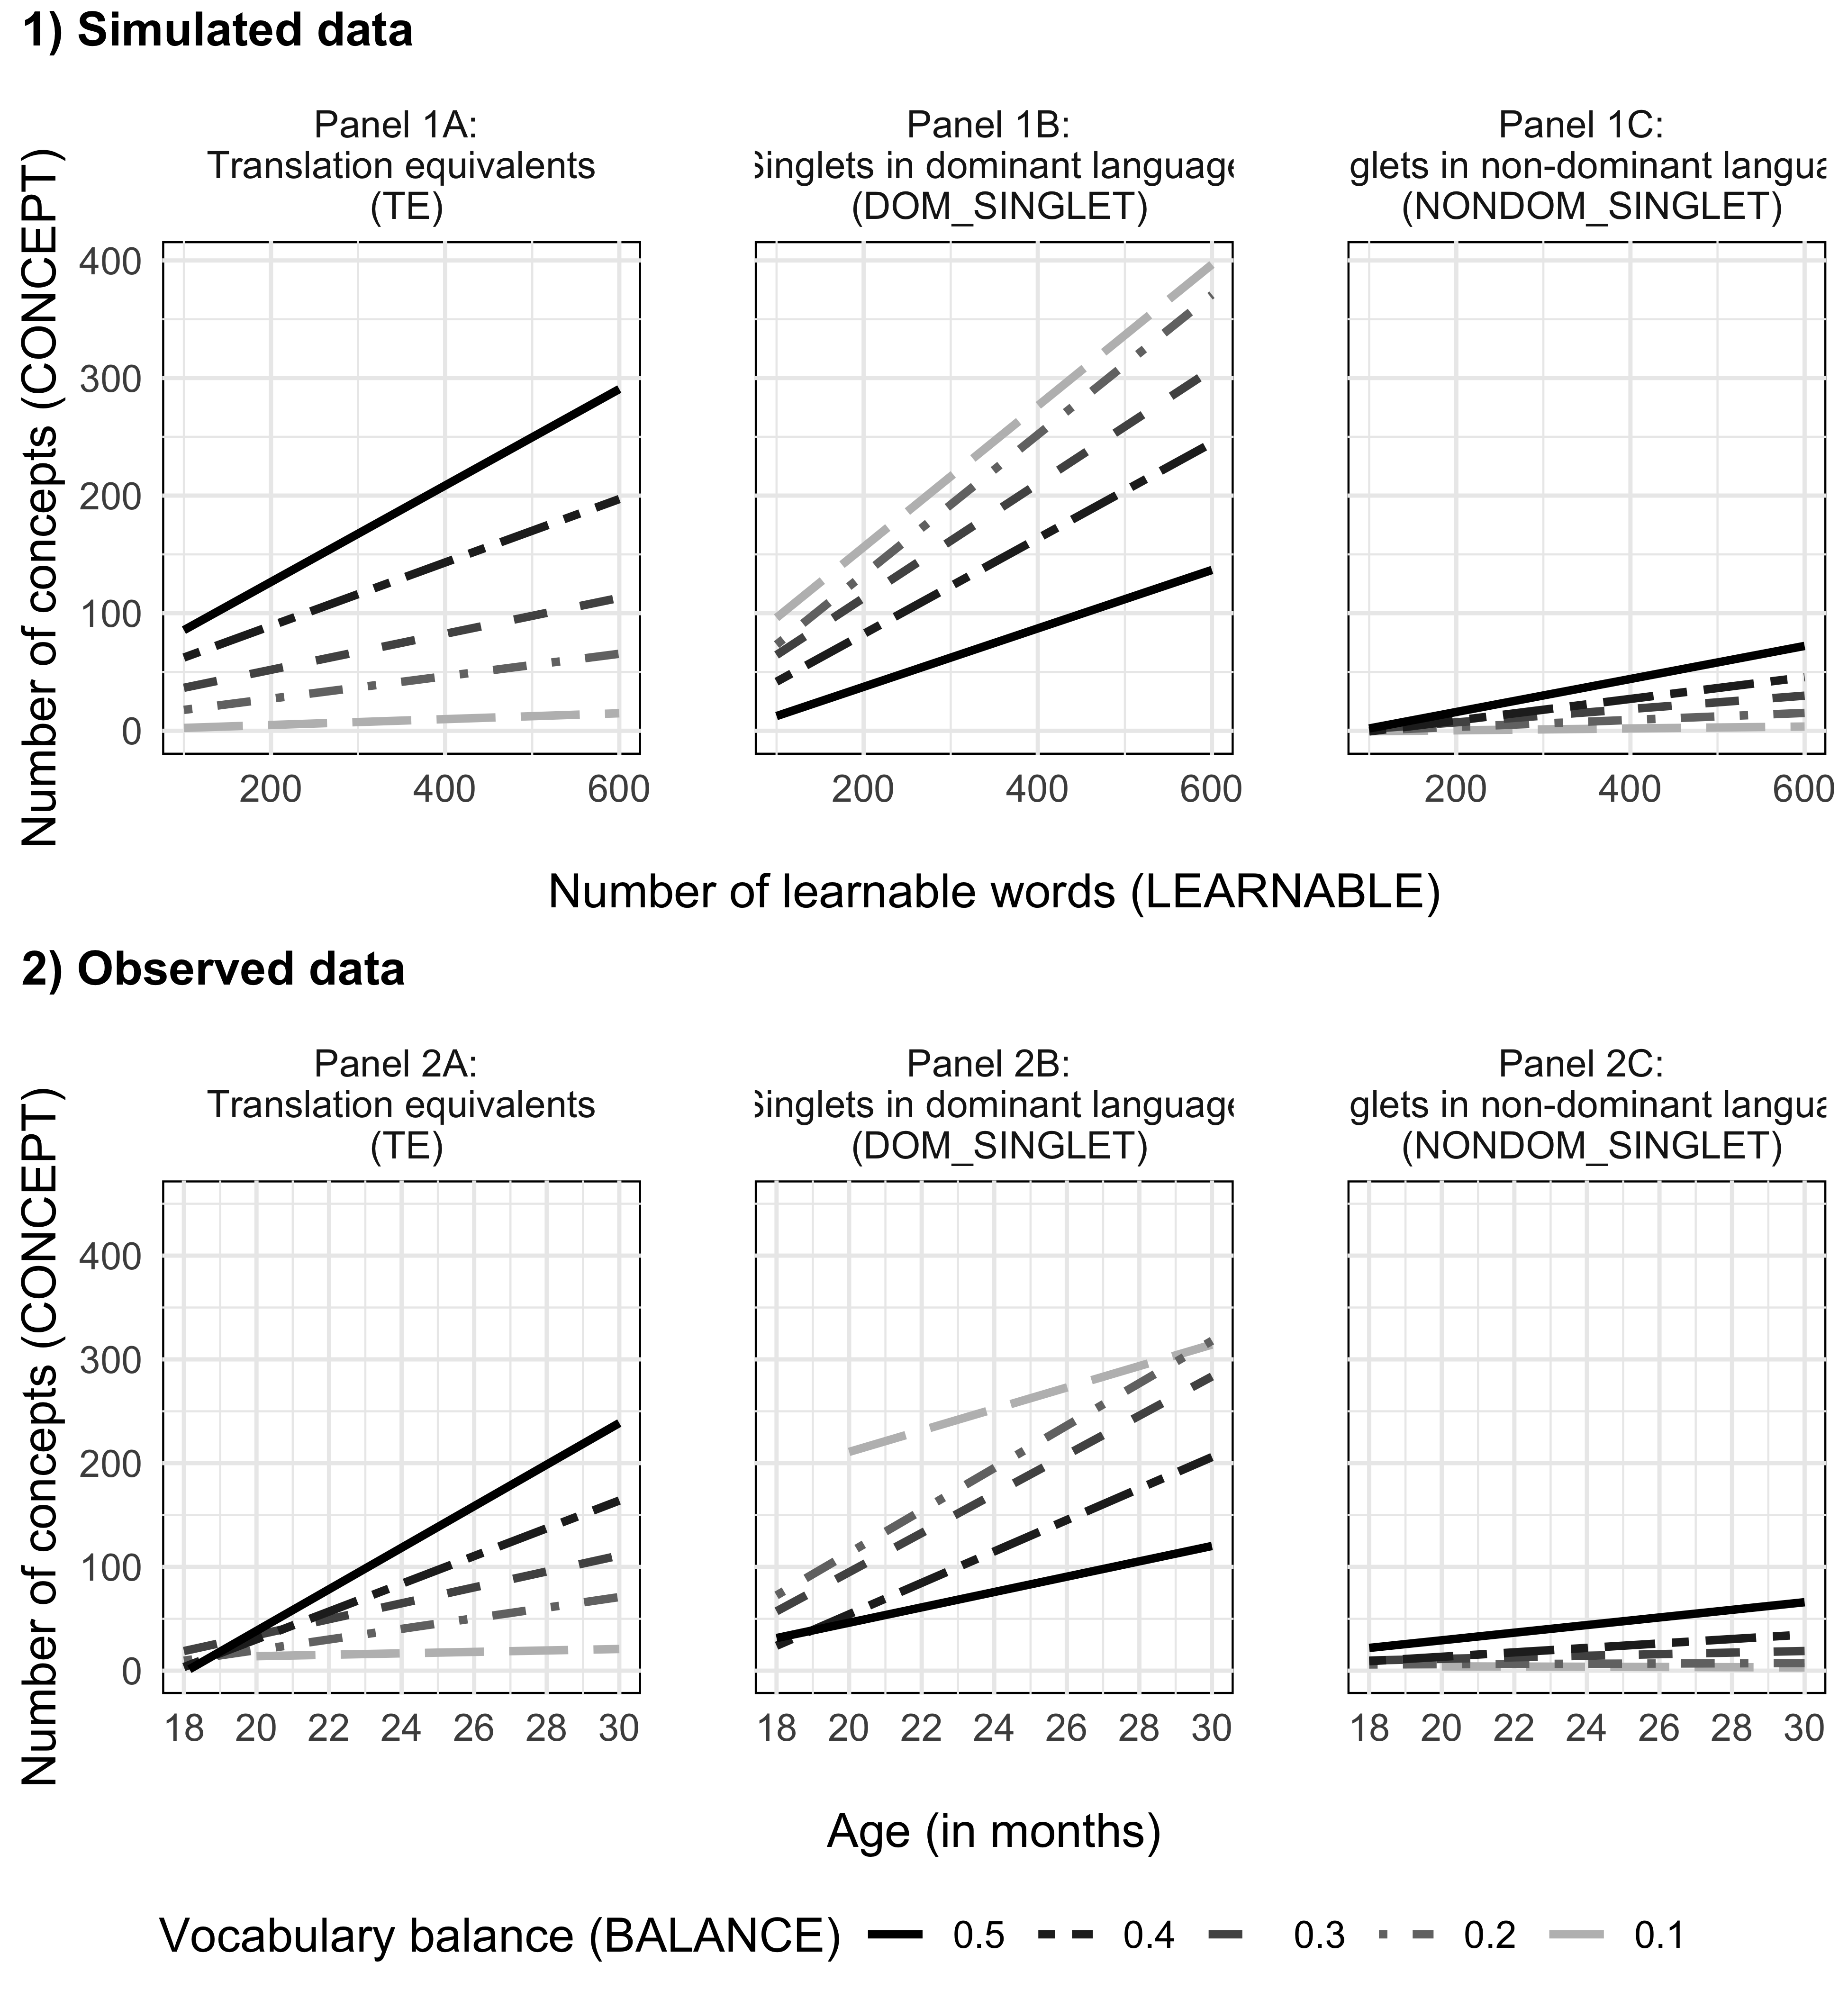
\includegraphics[width=1\linewidth]{paper_TE_bilingual_vocabulary_model_files/figure-latex/fig2-1} 

}

\caption{Number of concept vocabulary (CONCEPT; Panel A), translation equivalents (TE; Panel B), singlets in dominant (DOM-SINGLET; Panel C) and singlets in the non-dominant language (NONDOM-SINGLET; Panel D) across different levels of vocabulary balance (BALANCE) in relation to different developmental levels/ages, which sets the number of LEARNABLE words. Row 1 represents the simulated data in Study 1. Row 2 represents the observed vocabulary data in Study 2.}\label{fig:fig2}
\end{figure}

\hypertarget{simulation-3-bias-towards-or-against-translation-equivalent-learning-compared-to-singlets}{%
\subsection{1.3 Simulation 3: Bias towards or against translation equivalent learning compared to singlets}\label{simulation-3-bias-towards-or-against-translation-equivalent-learning-compared-to-singlets}}

In Simulations 1 and 2, we modeled cases in accordance with the Neutral Account where dominant-language and non-dominant language words were learned independently, such that the bias parameter (BIAS) was exactly 1 when we calculated TE as DOM×NONDOM/LEARNABLE. In our final simulation, we examined cases where dominant-language and non-dominant language words were not independent, corresponding to the Avoidance Account and the Preference Account. Mathematically, this requires varying the BIAS parameter. For the Preference Account, BIAS will be greater than 1, meaning that TEs are more easily learned than singlets. By contrast, for the Avoidance Account, BIAS will be less than 1, meaning that TEs are less easily learned than singlets.

Translation equivalent (TE) knowledge was first simulated across different developmental levels (as indicated by number of LEARNABLE words = 150, 300, 450, 600), in conjunction with a wide range of values for DOM and NONDOM. Again, BALANCE and word vocabulary (WORD) were calculated based on the values of DOM and NONDOM. The final simulated data set contained 166 data points (see Table 2 for a summary of the parameters used). Three scenarios of translation equivalent learning (TE) were then generated using the formula TE = BIAS × DOM×NONDOM/LEARNABLE. To illustrate the Avoidance Account, BIAS was set at .5 (i.e., TEs are 50\% less likely to be learned than singlets). To illustrate the Neutral Account, BIAS was set at 1 (i.e., TEs are equally learnable as singlets). Finally, to illustrate the Preference Account, BIAS was set at 1.5 (i.e., TE are 50\% more likely to be learned than singlets). In Figure 3, we illustrate the three different scenarios of simulated translation equivalent (TE) knowledge. Again, we observed a pattern consistent with prediction 1a where, in all cases, simulated children with more balanced vocabularies (BALANCE) produced more translation equivalents (TE). Thus, overall relationships between BALANCE and TE remained similar across the Avoidance, Preference, and Neutral Accounts. What changed was the slope of translation equivalent learning: the slopes were the shallowest under the Avoidance Account where BIAS = 0.5, whereas the slopes were steepest under the Preference Account where BIAS = 1.5. With this, we further outline Prediction Set 3:

\begin{itemize}
\tightlist
\item
  Prediction 3: Whether translation equivalents are harder to learn, easier to learn, or similar to learn as singlets will change the slope of translation equivalent learning as a function of word vocabulary (WORD), with a shallower slope if TEs are less easily learned (i.e., Avoidance Account), and a steeper slope if TEs are more easily learned (i.e., Preference Account) compared to where translation equivalents are similar to learn as singlets (i.e., Neutral Account).
\end{itemize}

\begin{figure}[H]

{\centering 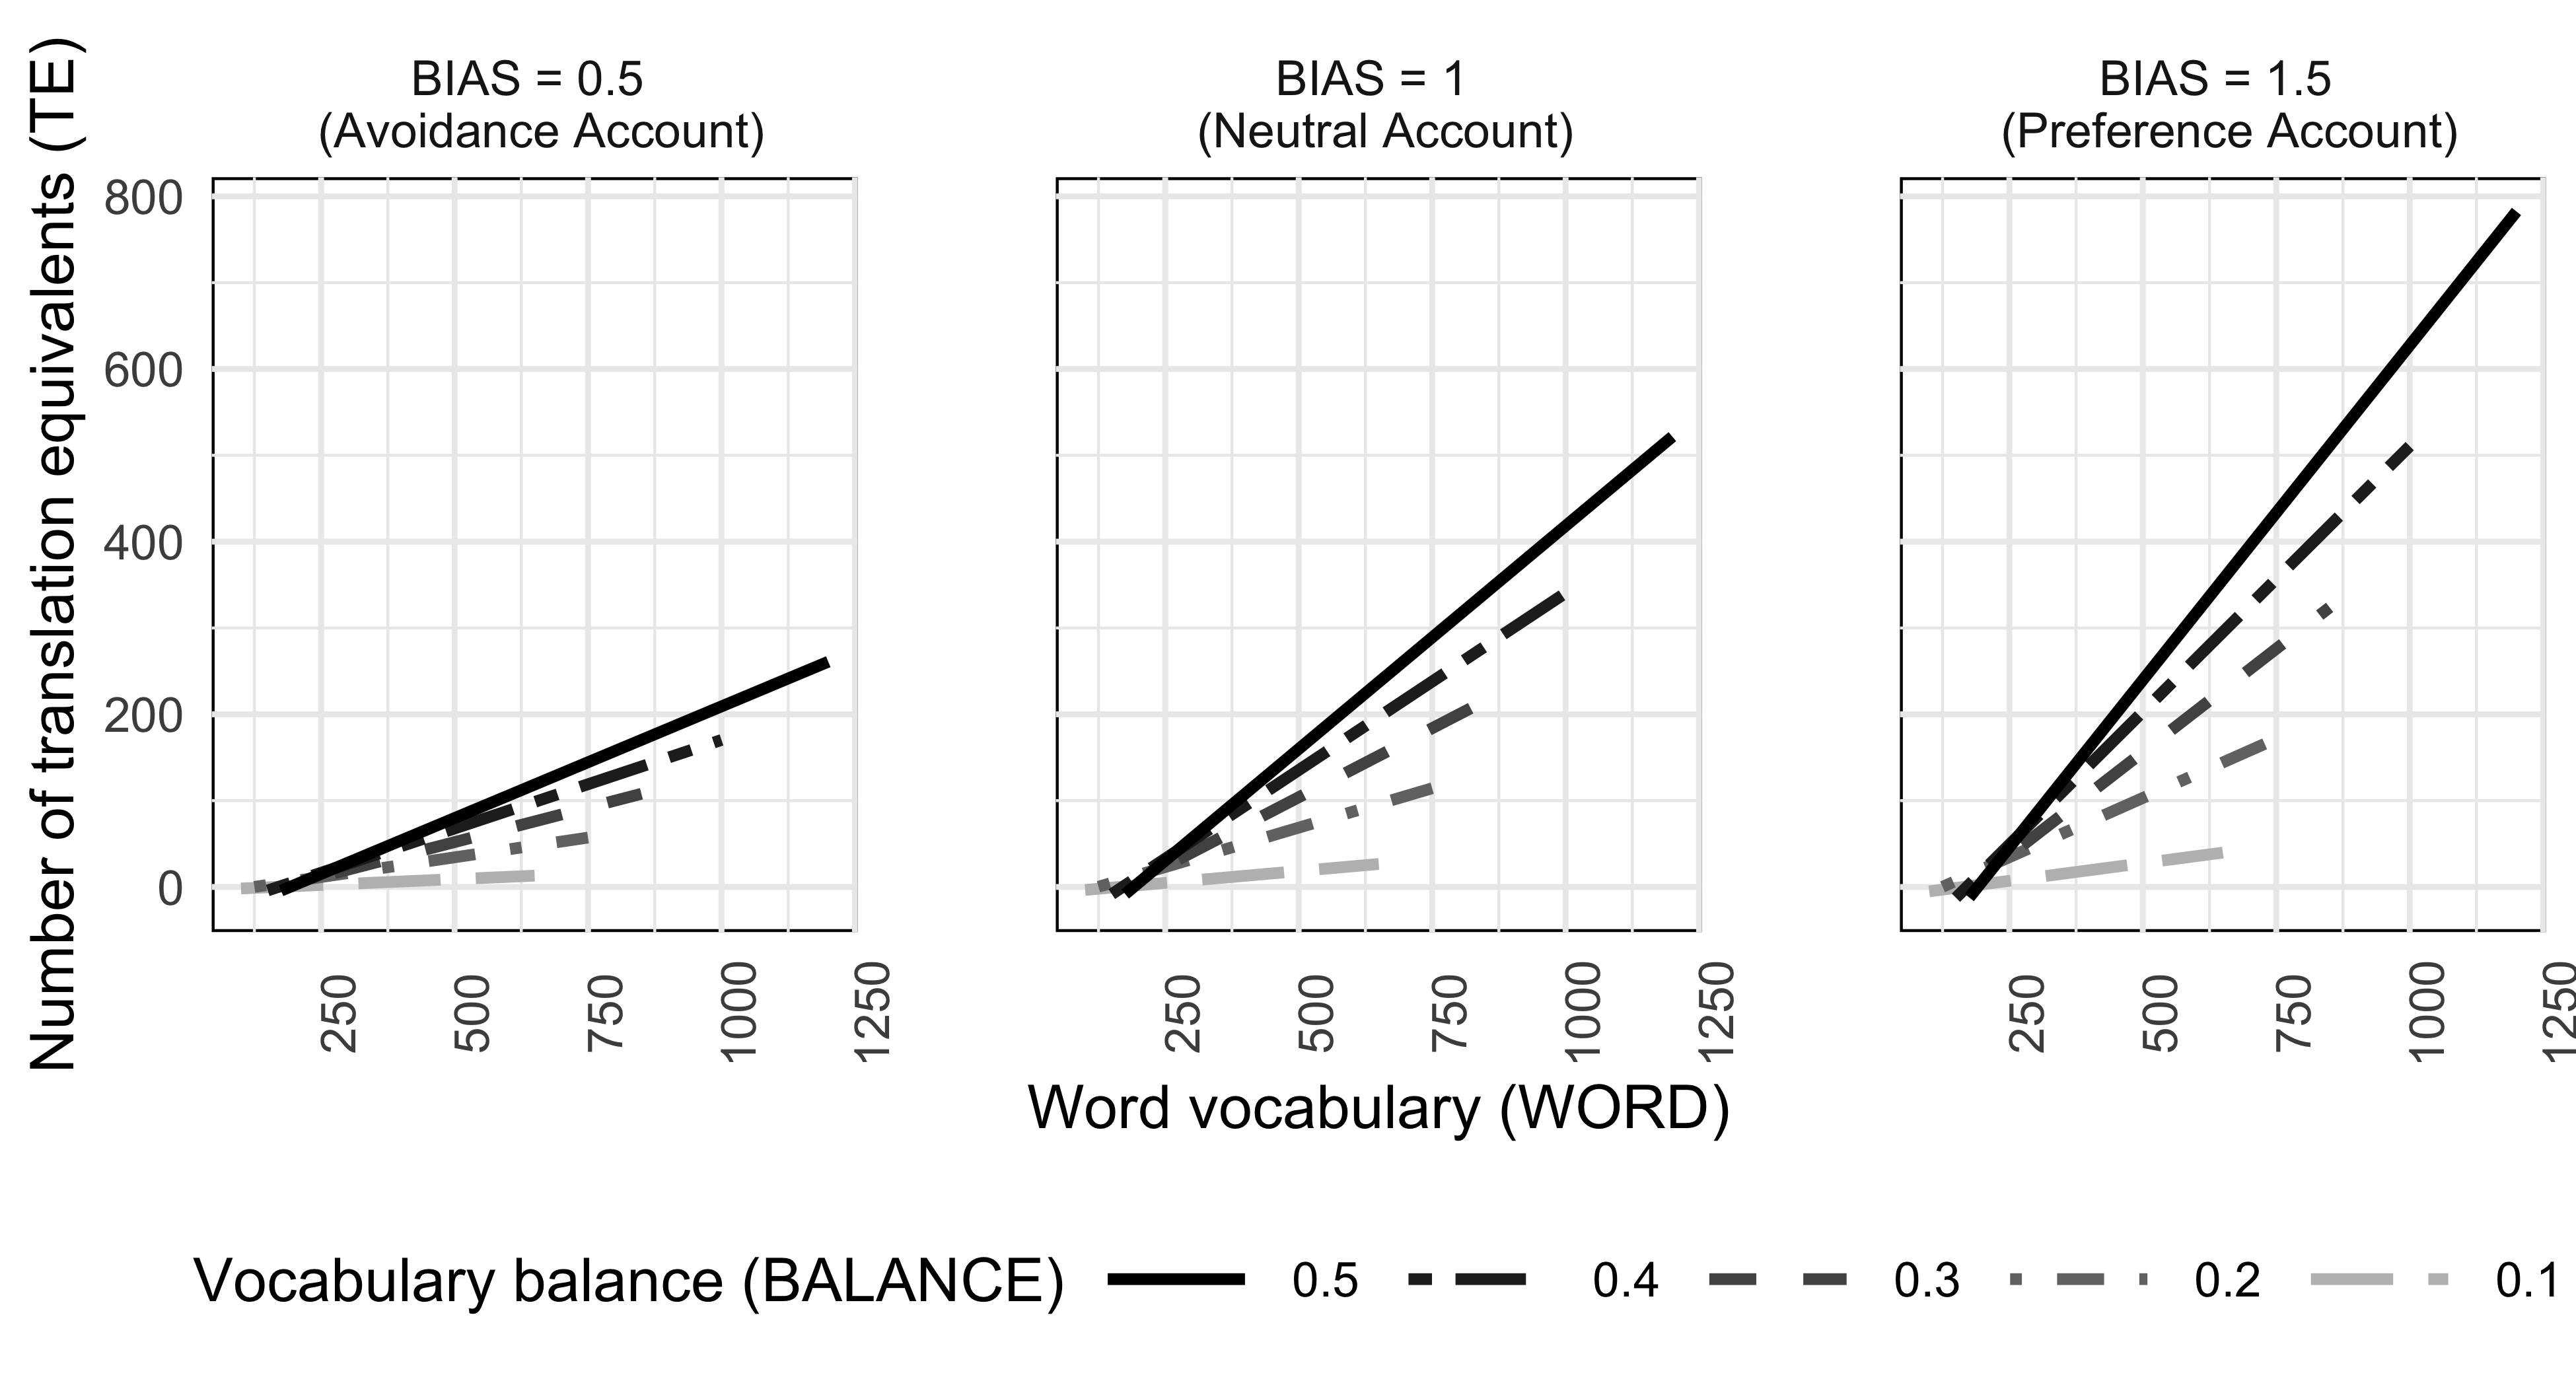
\includegraphics[width=1\linewidth,height=0.8\textheight]{paper_TE_bilingual_vocabulary_model_files/figure-latex/fig3-1} 

}

\caption{Different scenarios of expected translation equivalents learning (TE) as a function of WORD vocabulary, under scenarios where TEs are harder to learn (BIAS < 1), easier to learn (BIAS > 1), or similar to learn (BIAS = 1) as singlets.}\label{fig:fig3}
\end{figure}

\hypertarget{summary-of-model-predictions}{%
\subsection{1.4 Summary of model predictions}\label{summary-of-model-predictions}}

Study 1 presented predictions under the Bilingual Vocabulary Model with regards to the effect of vocabulary sizes and developmental variables on translation equivalent learning. Assuming that translation equivalents were learned similarly to singlets (i.e., the Neutral Account), three sets of predictions were made. Prediction Set 1 illustrated that the more words children produce in total vocabulary, their dominant language, or the non-dominant language, the more translation equivalents they are predicted to produce. Moreover, children with more balanced vocabularies (i.e., producing a similar number of words in each of their languages) are also expected to produce more translation equivalents. Prediction Set 2 described translation equivalent knowledge in relation to the number of learnable words constrained by a child's developmental level. Older children are predicted to produce more concept vocabularies including translation equivalents and singlets in both dominant and non-dominant languages than younger children. Moreover, the most balanced children are expected to produce more singlets in their non-dominant language, whereas the least balanced children are expected to produce more singlets in their dominant language. Finally, Prediction Set 3 quantitatively demonstrated the patterns of translation equivalent learning under the three different accounts: the Avoidance Account, the Preference Account, and the Neutral Account. Crucially, these predictions should not be thought of as fully independent from each other, but instead illustrate the interrelatedness of measures of bilingual vocabulary under the Bilingual Vocabulary Model. In Study 2, we used vocabulary data from bilingual infants to investigate whether these same patterns of interrelatedness would be observed, thus validating our model.

\hypertarget{study-2-empirical-data}{%
\section{Study 2: Empirical data}\label{study-2-empirical-data}}

In Study 1, we used a simulation based on the Bilingual Vocabulary Model to generate several predictions about the relationship between translation equivalent knowledge and other vocabulary variables. In Study 2, we tested these predictions using archival vocabulary data from 200 French--English bilingual children aged 18 to 33 months.

\hypertarget{method}{%
\subsection{2.1 Method}\label{method}}

Ethics approval was obtained by the Human Research Ethics Board of Concordia University (Certificate Number 10000439) and informed consent was obtained from the children's parents.

\hypertarget{participants}{%
\subsection{2.1.1 Participants}\label{participants}}

Archival data from 200 bilingual children acquiring English and French (age range: 18.40 - 33.50 months; 94 girls and 106 boys) who participated in prior studies at Concordia Infant Research Lab were included in the present study, drawn from the same set of participants as Gonzalez-Barrero et al.~(2020). Data collection was conducted in Montréal, Québec, Canada. Montréal is a multicultural city where both English and French are widely used in society. Some children took part in more than one in-lab study (n = 28); thus, they contributed data at more than one time point. This resulted in a larger number of datapoints relative to the number of unique participants. The total number of data points included in the analyses was 229 (i.e., 229 English and 229 French CDI questionnaires). Participants were recruited through government birth lists, online ads, daycares, and infant-parent group activities (e.g., children's library activities). Inclusion criteria were the following: full term-pregnancy ( i.e., \textgreater{} 36 weeks of gestation), normal birth weight (\textgreater{} 2500 grams), and absence of major medical conditions (i.e., meningitis). Only children who had complete data in both CDI forms (i.e., English and French) were retained for analysis. Bilingual children were defined as those exposed at least 25\% of the time over the course of their lives globally to both English and French and with less than 10\% of exposure to a third language. For children who participated more than once, their language exposure followed such criteria for all visits. Following the approach in Study 1, children's dominant language was deemed to be the language in which the child produced a greater number of words; vocabulary balance was then determined based on the proportion of words produced in the non-dominant language relative to the total words produced across both languages using the same formula as in Study 1: NONDOM/(DOM+NONDOM). Within the 229 data points, 59.80\% of children were English-dominant and 40.20\% were French-dominant. Children's demographic characteristics including age, maternal education, and language exposure, are presented in Table 4.

~

\begin{table}[h]

\begin{center}
\begin{threeparttable}

\caption{\label{tab:table4}Table 4. Demographic characteristics of participants (data points = 229).}

\begin{tabular}{lccc}
\toprule
 & Mean & $SD$ & Range\\
\midrule
Age in months & 24.4 & 4.7 & 18.4 - 33.5\\
Maternal education in years & 16.6 & 2.1 & 10 - 21\\
\% Global exposure to English & 51.7 & 14.8 & 25 - 75\\
\% Global exposure to French & 47.8 & 15.0 & 25 - 75\\
\% Global exposure to Other & 0.6 & 1.8 & 0 - 10\\
\bottomrule
\end{tabular}

\end{threeparttable}
\end{center}

\end{table}

\hypertarget{measures}{%
\subsection{2.1.2 Measures}\label{measures}}

\hypertarget{macarthur-bates-communicative-development-inventories-words-and-sentences-cdi}{%
\subsubsection{MacArthur-Bates Communicative Development Inventories: Words and Sentences (CDI)}\label{macarthur-bates-communicative-development-inventories-words-and-sentences-cdi}}

Bilingual children's expressive vocabulary was measured by the Words and Sentences form of the MacArthur-Bates CDI. Caregivers completed the original CDI English version (Fenson et al., 2007) and its Québec French adaptation (Trudeau et al., 1999). We asked the caregiver more familiar with each language to complete the respective CDI form, and the forms are mainly filled out by mothers (64\%), fathers (7\%), both parents (4\%), others (\textless{} 1\%; e.g., grandmother), or else the respondent was not indicated (24\%). In some cases different caregivers filled out each form, while in other cases the same caregiver filled out both forms. Our analyses focused on the vocabulary checklist of this questionnaire, which includes different nouns, verbs, adjectives, and other words used by young children. There are 680 words on the English CDI version and 664 in the Québec French version.

Translation equivalents (TE) were determined in the same manner as Gonzalez-Barrero et al.~(2020) by three proficient bilingual French--English adults who carefully examined each language version of the CDI. Word pairs that made reference to the same concept (e.g., English ``apple'' and French \emph{``pomme''}) were considered to be translation equivalents. In cases of disagreement, a discussion of the likely uses of the word in question by children (rather than potential adult uses of the word) was conducted and then a decision was made. Words that had similar phonetic realizations (e.g., English ``alligator'' and French \emph{``alligator''}) were also considered translation equivalents. Most of the items on both vocabulary checklists had an equivalent word in the other language, which resulted in a total of 611 translation equivalents. A full list of translation equivalents is available at \url{https://osf.io/2t5kw/}.

After determining the dominant language of a child based on the vocabulary size, we then computed the number of singlets that children knew in their dominant (DOM-SINGLET) and non-dominant (NONDOM-SINGLET) languages by deducting the number of translation equivalents produced from the total number of words produced in each language (i.e., DOM - TE and NONDOM - TE as in Study 1). Concept vocabulary (CONCEPT) was computed based on the number of concepts for which a child produced a word, calculated by subtracting the number of translation equivalents from word vocabulary (i.e., WORD - TE as in Study 1).

\hypertarget{language-exposure-questionnaire-using-the-maple-approach}{%
\subsubsection{Language Exposure Questionnaire using the MAPLE approach}\label{language-exposure-questionnaire-using-the-maple-approach}}

Children's language exposure was measured using the Language Exposure Questionnaire (LEQ; Bosch \& Sebastián-Gallés, 2001) and the Multilingual Approach to Parent Language Estimates (MAPLE; Byers-Heinlein et al., 2020). The LEQ is a structured interview that lasts approximately 15 minutes. It includes targeted questions that quantify the child's language exposure from birth until their current age. The LEQ and MAPLE provide a global language exposure estimate based on the number of hours the child is exposed to each language within all contexts (e.g., home, daycare, etc.). Children's average global exposure to each language is described in Table 4.

\hypertarget{procedure}{%
\subsection{2.1.3 Procedure}\label{procedure}}

Caregivers were asked to fill out the CDI questionnaires as part of their child's participation in experimental studies on language development, speech perception, and word learning. Caregivers were instructed to check off the words produced by their child using either a CDI paper questionnaire or the same questionnaire administered on a tablet. Data from paper based questionnaires were double entered and checked by trained research assistants.

\hypertarget{results}{%
\subsection{2.2 Results}\label{results}}

Data analyses were conducted using R (Version 4.0.2, 2020). Analysis scripts and the data set used in the present study are available at \url{https://osf.io/2t5kw/}. We first present descriptive measures of vocabulary, and then tests of the three sets of predictions generated in Study 1.

\hypertarget{descriptive-measures-of-vocabulary}{%
\subsection{2.2.1 Descriptive measures of vocabulary}\label{descriptive-measures-of-vocabulary}}

On average, bilinguals in the sample had a mean word vocabulary size (WORD) of 295 (SD = 254.60), with a wide range of 6 - 1071 words. As expected by the way language dominance was defined, children produced more words in their dominant language (DOM; M = 206.10, SD = 175.60, range = 4 - 657) than in their non-dominant language (NONDOM; M = 88.90, SD = 98.50, range = 2 - 469), \emph{t}(228) = 13.89, \(p < .001\), \(d = 0.92\).

Children produced an average of 67.70 translation equivalents (TE; SD = 85.10, range = 1 - 409). The remainder of words were singlets, and children produced many more singlets in their dominant language (DOM-SINGLET; M = 138.40, SD = 124.40, range = 2 - 523) than in their non-dominant language (NONDOM-SINGLET; M = 21.20, SD = 20.10, range = 0 - 94), \emph{t}(228) = 13.89, \(p < .001\), \(d = 0.92\). On average, children's concept vocabulary size was 227.30 words (CONCEPT; SD = 181.30, range = 4 - 695).

Vocabulary balance (BALANCE) was then determined based on the proportion of total words produced in the non-dominant language following the formula BALANCE = NONDOM/WORD as in Study 1. On average, bilingual children in our sample had a balance score BALANCE of 0.31 (SD = 0.13), ranging from 0.02 to 0.50. Similar vocabulary balance was found between the children who were English-dominant and those who were French-dominant, \emph{t}(200.43) = 0.57, \(p = .566\), \(d = 0.08\). The 59.80\% of children who were English-dominant had an average BALANCE of 0.31 (SD = 0.13, range = 0.02 - 0.50) whereas the remaining 40.20\% who were French-dominant had an average BALANCE of 0.30 (SD = 0.12, range = 0.05 - 0.50).

Note that in this paper, we defined BALANCE in terms of relative vocabulary in each language, which numerous studies have found is related to children's relative input in each language (e.g., David \& Wei, 2008; Pearson et al., 1997; Hurtado et al., 2013). We therefore investigated the relationship between vocabulary balance and the percent of exposure bilingual children received in their non-dominant language. For most children, the language in which they produced the most words was also the language that they heard most often (181 children, 79\%), although this was not the case for a minority of children (48 children, 21\%). The correlation between BALANCE and the percentage of exposure to the non-dominant language was moderate, \emph{r}(227) = 0.45, \(p < .001\) (see also Figure 4). The imperfect correlation between these two measures could result from measurement error (see Byers-Heinlein et al., 2021, for a discussion of attenuation of correlation due to measurement error in developmental research) or could also be because vocabulary size in each language is determined by factors beyond parent-reported proportion of input in each language, for example the quality of that input (for a discussion of input quality for bilinguals, see Unsworth, 2016).

~

\begin{figure}[H]

{\centering 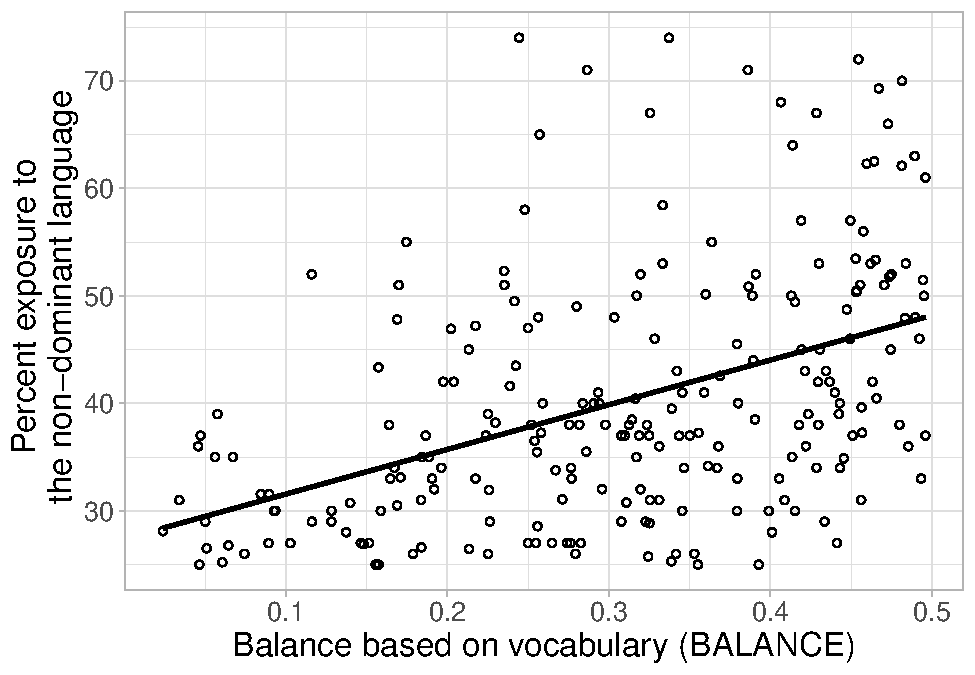
\includegraphics[width=0.75\linewidth]{paper_TE_bilingual_vocabulary_model_files/figure-latex/fig4-1} 

}

\caption{Correlation between balance defined by vocabulary (BALANCE) and balance defined by exposure.}\label{fig:fig4}
\end{figure}

\hypertarget{testing-prediction-set-1-univariate-relationships-between-translation-equivalents-and-different-vocabulary-measures}{%
\subsection{2.2.2 Testing Prediction Set 1: Univariate relationships between translation equivalents and different vocabulary measures}\label{testing-prediction-set-1-univariate-relationships-between-translation-equivalents-and-different-vocabulary-measures}}

Prediction Set 1 pertained to the pairwise relationships between word vocabulary (WORD), dominant (DOM) and non-dominant vocabulary (NONDOM), vocabulary balance (BALANCE), and translation equivalents (TE), which we examined through Pearson's correlations. Overall, the univariate statistics showed strong correspondence with the relationships predicted by Prediction 1 under the Bilingual Vocabulary Model (see Table 5 for a full table of pairwise correlations\footnote{Note that there was a negative correlation between BALANCE and age in our sample. We believe that this could be related to patterns of language exposure at child care (i.e., attending childcare in one language could have made exposure less balanced), which is not related to our model per se.}).

Prediction 1a was that children with more balanced vocabularies would produce more translation equivalents. As shown in Figure 1 Row 2 (Observed data), our vocabulary data confirmed the prediction, \emph{r}(227) = 0.25, \(p < .001\), where children with the most balanced vocabulary produced the most translation equivalents.

Prediction 1b was that children with larger word vocabularies and larger dominant-language vocabularies would produce more translation equivalents, and the results from our dataset confirmed this prediction, for word vocabulary (WORD): \emph{r}(227) = 0.90, \(p < .001\), and dominant-language vocabulary (DOM): \emph{r}(227) = 0.76, \(p < .001\). Figure 1 Panels 2A and 2B further illustrates these relationships observed in our dataset.

Prediction 1c was that children who produce more words in the non-dominant language (NONDOM) would produce more translation equivalents (TE), specifically that this relationship would be nearly perfect. As shown in Figure 1 Panel 2C, we observed that these two variables were indeed nearly perfectly correlated, \emph{r}(227) = 0.99, \(p < .001\).

\begin{lltable}

\begin{TableNotes}[para]
\normalsize{\textit{Note.} *** p < .001, ** p < .01, * p < .05.}
\end{TableNotes}

\scriptsize{

\begin{longtable}{llllllllll}\noalign{\getlongtablewidth\global\LTcapwidth=\longtablewidth}
\caption{\label{tab:table5}Table 5. Pairwise correlations among variables (corrected for multiple comparisons using Benjamini and Yekutieli [2001]).}\\
\toprule
 & \multicolumn{1}{c}{LEARNABLE} & \multicolumn{1}{c}{BALANCE} & \multicolumn{1}{c}{WORD} & \multicolumn{1}{c}{DOM} & \multicolumn{1}{c}{NONDOM} & \multicolumn{1}{c}{TE} & \multicolumn{1}{c}{DOM-SINGLET} & \multicolumn{1}{c}{NONDOM-SINGLET} & \multicolumn{1}{c}{CONCEPT}\\
\midrule
\endfirsthead
\caption*{\normalfont{Table \ref{tab:table5} continued}}\\
\toprule
 & \multicolumn{1}{c}{LEARNABLE} & \multicolumn{1}{c}{BALANCE} & \multicolumn{1}{c}{WORD} & \multicolumn{1}{c}{DOM} & \multicolumn{1}{c}{NONDOM} & \multicolumn{1}{c}{TE} & \multicolumn{1}{c}{DOM-SINGLET} & \multicolumn{1}{c}{NONDOM-SINGLET} & \multicolumn{1}{c}{CONCEPT}\\
\midrule
\endhead
Age (in month) & 0.96*** & -0.24*** & 0.65*** & 0.69*** & 0.45*** & 0.48*** & 0.65*** & 0.19** & 0.69***\\
LEARNABLE &  & -0.23*** & 0.62*** & 0.66*** & 0.43*** & 0.45*** & 0.63*** & 0.21** & 0.67***\\
BALANCE &  &  & -0.07 & -0.29*** & 0.35*** & 0.25*** & -0.58*** & 0.63*** & -0.21**\\
WORD &  &  &  & 0.96*** & 0.87*** & 0.90*** & 0.74*** & 0.44*** & 0.98***\\
DOM &  &  &  &  & 0.70*** & 0.76*** & 0.89*** & 0.23*** & 0.99***\\
NONDOM &  &  &  &  &  & 0.99*** & 0.31*** & 0.72*** & 0.76***\\
TE &  &  &  &  &  &  & 0.38*** & 0.60*** & 0.80***\\
DOM-SINGLET &  &  &  &  &  &  &  & -0.09 & 0.86***\\
NONDOM-SINGLET &  &  &  &  &  &  &  &  & 0.33***\\
CONCEPT &  &  &  &  &  &  &  &  & \\
\bottomrule
\addlinespace
\insertTableNotes
\end{longtable}

}

\end{lltable}

\hypertarget{testing-prediction-set-2-the-vocabulary-composition-of-bilingual-children-at-different-developmental-levels}{%
\subsection{2.2.3 Testing Prediction Set 2: The vocabulary composition of bilingual children at different developmental levels}\label{testing-prediction-set-2-the-vocabulary-composition-of-bilingual-children-at-different-developmental-levels}}

Prediction Set 2 pertained to expected patterns of acquisition of translation equivalents and singlets for children of different developmental levels. In our data set, developmental level was approximated by children's age. Figure 2 Panel B shows the number of concept vocabulary (CONCEPT), translation equivalents (TE), singlets in the dominant language (DOM-SINGLET) and in the non-dominant language (NONDOM-SINGLET) of the bilingual children as a function of different ages (our proxy for developmental level), used to estimate the number of LEARNABLE words.

Prediction 2a was that older children (i.e., those at a later developmental level) would have larger concept vocabularies than younger children (i.e., those at an earlier developmental level). As shown in Figure 2 Panel 2A, we observed a positive correlation between age (used as a proxy for developmental level, which determines LEARNABLE) and concept vocabulary (CONCEPT) in our dataset, \emph{r}(227) = 0.69, \(p < .001\), and therefore confirmed the prediction.

Prediction 2b was that older children would produce more translation equivalents than younger children. As illustrated in Figure 2 Panel 2B, we observed a positive correlation between age (our proxy for LEARNABLE) and number of translation equivalents in our dataset, \emph{r}(227) = 0.48, \(p < .001\), and therefore confirmed the prediction.

Prediction 2c was that both older children and those with the least balanced vocabularies (BALANCE) would produce more dominant-language singlets (DOM-SINGLET). This pattern was confirmed by the results from our dataset, with a positive correlation between dominant-language singlets (DOM-SINGLET) and age (which determined LEARNABLE), \emph{r}(227) = 0.65, \(p < .001\), and a negative correlation between BALANCE and dominant-language singlets (DOM-SINGLET), \emph{r}(227) = -0.58, \(p < .001\). This is illustrated in Figure 2 Panel 2C.

Prediction 2d was that older children and those with the most balanced vocabularies (BALANCE) would produce more singlets in their non-dominant language. This pattern was also observed in our dataset, with a positive correlation between the number of non-dominant singlets (NONDOM-SINGLET) and age (which determined LEARNABLE), \emph{r}(227) = 0.19, \(p = .005\), and a positive correlation between BALANCE and the number of non-dominant singlets (NONDOM-SINGLET), \emph{r}(227) = 0.63, \(p < .001\). This is illustrated in Figure 2 Panel 2D.

\hypertarget{testing-prediction-set-3-rate-of-translation-equivalent-learning}{%
\subsection{2.2.4 Testing Prediction Set 3: Rate of translation equivalent learning}\label{testing-prediction-set-3-rate-of-translation-equivalent-learning}}

Prediction Set 3 pertained to the overall nature of translation equivalent learning, describing expected patterns of translation equivalent learning under the Neutral Account, the Avoidance Account, or the Preference Account. To directly test the correspondence of our data with these different accounts, we built a linear regression model predicting the observed number of translation equivalents from the Bilingual Vocabulary Model using the formula TE = DOM×NONDOM/LEARNABLE, and we allowed the model to estimate the BIAS parameter.

First, we will walk through the parameters in this model. The size of dominant vocabulary (DOM) and size of non-dominant vocabulary (NONDOM) were taken to be the number of words produced by individual children observed in the vocabulary data. Again, the number of learnable words (LEARNABLE) was determined by averaging English and French productive CDI vocabulary at the 90th percentile at different ages (percentile information obtained from Wordbank version 0.3.1; Frank et al., 2016). Table 6 lists the denominators derived from averaging these percentiles, or LEARNABLE, at different ages. For example, for an 18 month-old infant, the denominator was 240 words which was calculated by averaging the 259 English words and 220 French words, based on what 18-month-old children would typically produce at the 90th percentile. For children who were between 31 to 33 months in our dataset, the 90th percentile of 30-month-old children was used since 90th percentile information was available only up to 30 months. Finally, the intercept of the linear regression model was set at 0 since no translation equivalents are expected to be produced if a child does not know any dominant or non-dominant vocabulary (i.e., when the predictor variables are 0).

\begin{table}

\caption{\label{tab:table6}Table 6. The number of total English and French productive CDI vocabulary at the 90th percentile at different ages according to WordBank, and the average between the two which serves as the denominator in our computation model. Values are rounded to the nearest integer.}
\centering
\fontsize{10}{12}\selectfont
\begin{tabular}[t]{>{\centering\arraybackslash}p{75px}>{\centering\arraybackslash}p{125px}>{\centering\arraybackslash}p{125px}>{\centering\arraybackslash}p{125px}}
\toprule
Age (months) & Number of English words produced at 90th percentile & Number of French words produced at 90th percentile & Average (LEARNABLE)\\
\midrule
18 & 259 & 220 & 240\\
19 & 321 & 274 & 298\\
20 & 378 & 325 & 352\\
21 & 430 & 372 & 401\\
22 & 476 & 416 & 446\\
\addlinespace
23 & 517 & 456 & 486\\
24 & 553 & 492 & 522\\
25 & 583 & 525 & 554\\
26 & 610 & 554 & 582\\
27 & 633 & 580 & 606\\
\addlinespace
28 & 653 & 602 & 627\\
29 & 668 & 620 & 644\\
30 - 33 & 681 & 635 & 658\\
\bottomrule
\end{tabular}
\end{table}

To reproduce the Bilingual Vocabulary Model's formula TE = DOM×NONDOM/LEARNABLE, an interaction between dominant and non-dominant vocabulary was entered in the model, but main effects were not included (denoted in R by using a colon rather than an asterisk between the interacting predictors). Therefore, our final linear regression model equation was\footnote{Note that for the purposes of running the model in R, the formula was rearranged and entered as \emph{ObservedTE * 90th percentile of CDI items \textasciitilde{} 0 + Dominant vocabulary:Non-dominant vocabulary}.}:

\emph{ObservedTE \textasciitilde{} 0 + Dominant vocabulary:Non-dominant vocabulary/90th percentile of CDI items.}

With the observed number of translation equivalents as the dependent variable, the regression coefficient estimated by the model indicates how the BIAS parameter is related to the empirical vocabulary data, which in turn indicates whether bilingual children were biased towards or against learning translation equivalents. If the coefficient is close to 1, then there is no bias and translation equivalents are learned equally to other words (i.e., the Neutral Account). Otherwise, a coefficient less than 1 indicates a bias against learning translation equivalents where translation equivalents are less easily learned (i.e., the Avoidance Account), and a coefficient greater than 1 indicates a bias towards learning translation equivalents where translation equivalents are more easily learned (i.e., the Preference Account).

Our model showed an excellent model fit of \(R^2\) = 0.96, indicating that our model explained 96\% of the variance in bilinguals' translation equivalent knowledge. BIAS coefficient was estimated at 1.04. This value is close to 1, suggesting that our data are consistent with the account whereby translation equivalents are learned equivalently to other words\footnote{We also explored how these results would vary if we set the number of LEARNABLE words at the 75th percentile, rather than at the 90th percentile. Overall, model fit was slightly reduced compared to our main model, although fit was still good, \(R^2\) = 0.95. The estimated BIAS parameter was lower, at 0.95, which is nonetheless still quite close to 1, and thus consistent with the Neutral Account. This change in the BIAS parameter is mathematically expected due to the reciprocal nature of LEARNABLE and BIAS, an issue we will return to in the discussion.}.

To illustrate the close fit between the Neutral Account and our data, we used the Bilingual Vocabulary Model formula TE = 1 × (DOM×NONDOM/LEARNABLE) to estimate each child's expected translation equivalent knowledge (setting BIAS = 1; also setting the intercept at 0 to replicate our linear regression model), which is plotted against our observed data in Figure 5. Expected and observed translation equivalents were closely aligned with the Neutral Account of the Bilingual Vocabulary Model (i.e., BIAS = 1), suggesting that the Neutral Account provides a parsimonious explanation for bilinguals' translation equivalent knowledge. This provides evidence for the notion that translation equivalents are neither harder nor easier to learn than singlets in bilingual vocabulary learning. Note that visual inspection suggested that there could be some possible outliers. Cook's distance was estimated for our linear regression model listed above and identified two data points with a cook's distance over 0.4. After removing those two data points, the linear regression model returned a coefficient of 1.07, with \(R^2\) = 0.96. As the model fit was similar to the model without eliminating the two outlier data points, we proceeded with the full data set keeping the two potential outlier data points.

\begin{figure}

{\centering 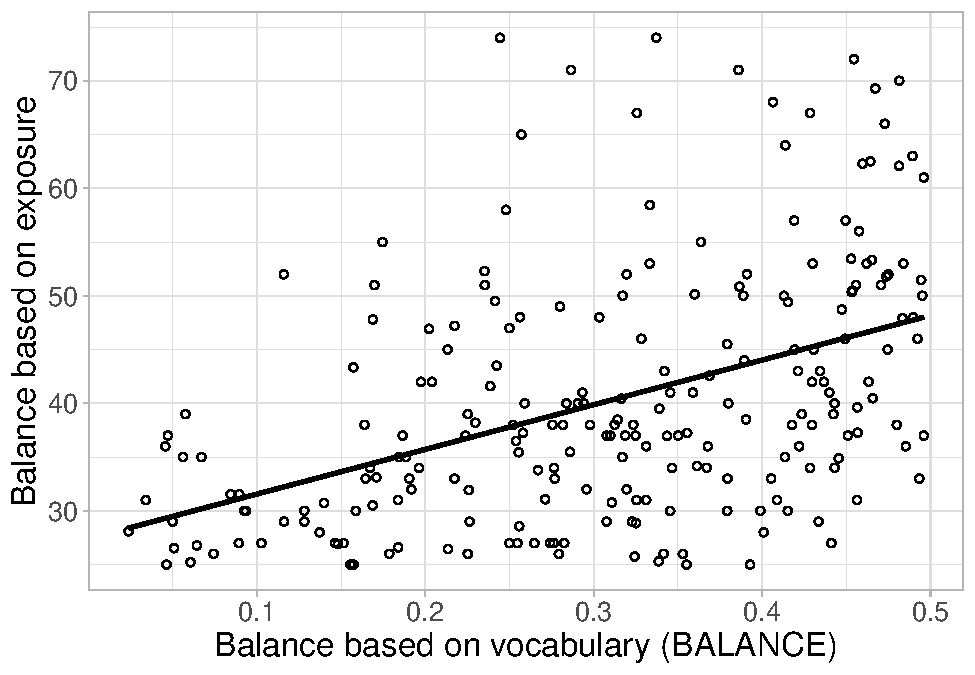
\includegraphics[width=0.6\linewidth,height=0.6\textheight]{paper_TE_bilingual_vocabulary_model_files/figure-latex/fig5-1} 

}

\caption{The number of simulated and observed translation equivalents plotted against each other. The dots represent the value of a child tested on the CDI, with their observed number of TEs and the expected number of TEs based on our model. The diagonal dashed line represents the case where the bias parameter equals 1 (BIAS = 1) such that the predicted and observed number of TEs are equal, and the solid blue line represents the model predictions.}\label{fig:fig5}
\end{figure}

Despite the good overall fit to the data, a close examination of Figure 5 suggested that the model might less closely fit the data of children with smaller vocabulary sizes. Figure 7 displays the model fit separately for children with a word vocabulary (WORD) less than 300 words and those with a word vocabulary (WORD) of 300 or greater. Based on visual inspection, the slope of translation equivalent learning appeared steeper for children with less than 300 total vocabulary, suggesting that translation equivalents are more easily learned (i.e., BIAS \textgreater{} 1); whereas the slope of translation equivalent learning appeared to align with the Neutral Account (i.e., BIAS = 1) for children with more than 300 total vocabulary. To further explore this pattern, we ran the same linear regression twice, separately for children with less than 300 total vocabulary and for those with more than 300 total vocabulary. The model for those with larger total word vocabulary (WORD) returned a coefficient of BIAS = 1.04, whereas the model for those with less than 300 total word vocabulary (WORD) returned a coefficient of BIAS = 2.21. Both models fit well, although a somewhat better fit was obtained for children with larger vocabulary size (\(R^2\) = 0.96) than children with smaller vocabulary size (\(R^2\) = 0.88). Overall, this analysis suggests that translation equivalent learning for children with larger vocabularies corresponds best to the Neutral Account, but translation equivalent learning for children with smaller vocabularies corresponds best to the Preference Account.

~

\begin{figure}

{\centering 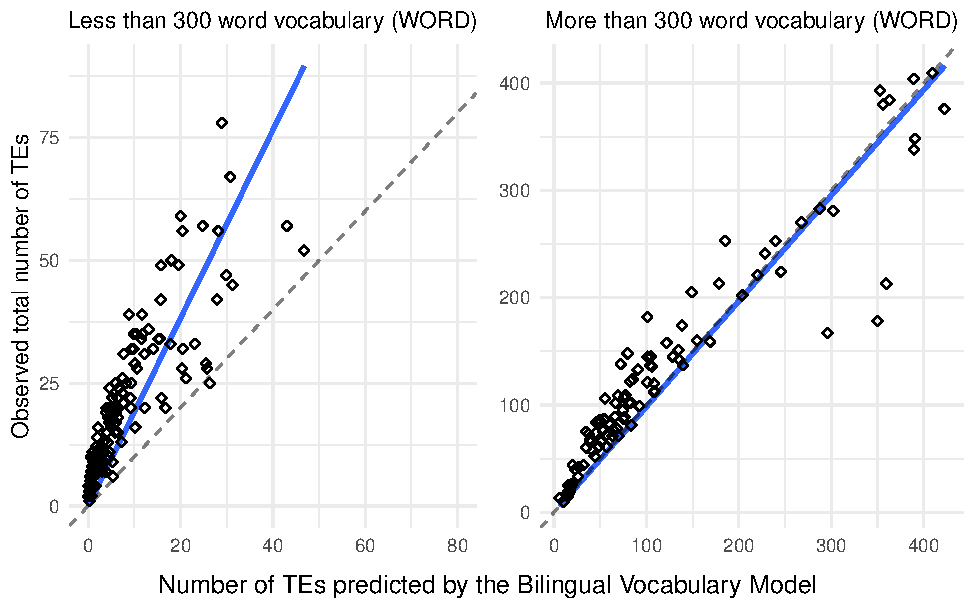
\includegraphics[width=1.2\linewidth]{paper_TE_bilingual_vocabulary_model_files/figure-latex/fig6-1} 

}

\caption{The number of observed translation equivalents as a function of number of expected translation equivalents under the Bilingual Vocabulary Model other (represented by the blue solid line), plotted separately for children with fewer than 300 word vocabulary (left panel) and for those with more than 300 word vocabulary (right panel). The dashed diagonal line represents the case where the parameter equals 1 (BIAS = 1) such that the predicted and observed number of TEs are equal.}\label{fig:fig6}
\end{figure}

\hypertarget{discussion}{%
\section{Discussion}\label{discussion}}

The aim of the current study was to better understand translation equivalent learning in bilingual children, specifically investigating whether translation equivalents are harder (Avoidance Account), easier (Preference Account), or similar (Neutral Account) for bilingual children to learn as singlet words (i.e., the first label for a particular referent). To test these accounts, we developed the Bilingual Vocabulary Model, which quantifies the number of translation equivalents that children produce as a product of words they know in their dominant and non-dominant language, divided by the number of words that are learnable at their developmental level. The inclusion of a learnability parameter was a unique aspect of our approach, and was crucial to quantifying how many translation equivalents versus singlets were possible to learn given the child's age. The relative difficulty of learning translation equivalents compared to singlets was modeled via a parameter that indicated whether translation equivalent learning was consistent with the Avoidance, Preference, or Neutral Account.

\hypertarget{confirmation-of-model-predictions}{%
\subsection{Confirmation of model predictions}\label{confirmation-of-model-predictions}}

In Study 1, we simulated vocabulary and translation equivalent knowledge based on the Bilingual Vocabulary Model, and in Study 2 we tested three sets of model-generated predictions using archival CDI data from 200 bilingual children aged 18-33 months. Three sets of model predictions were confirmed in our empirical dataset. In Table 7, we summarize the model predictions along with the evidence in our empirical dataset and findings in the literature.

\begin{landscape}\begin{table}

\caption{\label{tab:table7}Table 7. Summary of model predictions, similar evidence from previous literature, and whether our empirical data was consistent with the prediction.}
\centering
\fontsize{7}{9}\selectfont
\begin{tabular}[t]{>{\raggedright\arraybackslash}p{200px}>{\raggedright\arraybackslash}p{250px}>{\centering\arraybackslash}p{150px}}
\toprule
Model predictions & Evidence in previous literature & Did we observe the same pattern in our empirical data?\\
\midrule
1A: Children with more balanced vocabularies (BALANCE) will produce more translation equivalents (TE). & Children with more balanced vocabularies (i.e., those who produced a similar number of words in each of their languages) produced more translation equivalents (David \& Wei, 2008; Legacy et al., 2016; Montanari, 2010; Pearson et al., 1995; 1997). & Yes\\
1B: Children who produce more total words (WORD) or more dominant-language words (DOM) will produce more translation equivalents (TE). & The number of translation equivalents a bilingual child knows increases along with their total vocabulary size (Legacy et al., 2016; Montanari, 2010). 
 There is a positive correlation between bilingual children’s size of dominant language vocabulary and the proportion of translation equivalents (Legacy et al., 2016; Poulin-Dubois et al., 2013) & Yes\\
1C: Children who produce more non-dominant language words (NONDOM) will produce more translation equivalents (TE); but unlike for WORD and DOM this does not interact with BALANCE; instead, non-dominant vocabulary size will be an almost perfect predictor of translation equivalent knowledge & Vocabulary size in the non-dominant language was positively correlated with the proportion of translation equivalents known by the child (Legacy et al., 2016). & Yes\\
2A: Older children will have larger concept vocabularies (CONCEPT) than younger children. & Older children had larger concept vocabularies (Pearson et al., 1993). & Yes\\
2B: Older children will produce more translation equivalents (TE), regardless of vocabulary balance (BALANCE). & Older bilingual children knew more translation equivalents than younger children  (David \& Wei, 2008; Legacy et al., 2016) & Yes\\
\addlinespace
2C: Older children will produce more dominant-language singlet words (DOM-SINGLET). Moreover, those with the least balanced vocabulary (BALANCE) will produce the most DOM-SINGLET. & Bilingual children learned words in proportion to their relative exposure to each language (e.g., Boyce et al., 2013; Hoff et al., 2012; Marchman et al., 2010; Pearson et al., 1997; Place \& Hoff, 2011) & Yes\\
2D: Older children will produce more non-dominant-language singlets (NONDOM-SINGLET). Moreover, those with the most balanced vocabulary (BALANCE) will produce the most NONDOM-SINGLET. &  & \\
\bottomrule
\end{tabular}
\end{table}
\end{landscape}

A first set of predictions pertained to relations between translation equivalent knowledge, vocabulary balance, and vocabulary size in the dominant and non-dominant languages. In both the simulated and observed data, children with more balanced vocabularies (i.e., those who produced a similar number of words in each of their languages) produced more translation equivalents. This pattern is consistent with reports from previous research (David \& Wei, 2008; Legacy et al., 2016; Montanari, 2010; Pearson et al., 1995; 1997). Moreover, both the simulated and observed data showed that the children who produced more total words also produced more translation equivalents, which is in line with previous research showing that the number of translation equivalents a bilingual child knows increases along with their total vocabulary size (Legacy et al., 2016; Montanari, 2010). Additionally, both our simulated and observed data showed that the more words children produced in their dominant language, the more translation equivalents they also produced. This pattern is consistent with previous research reporting a positive correlation between bilingual children's size of dominant language vocabulary and the proportion of translation equivalents (Legacy et al., 2016; Poulin-Dubois et al., 2013). Finally, both our simulated and observed data showed that the more words children produced in their non-dominant language, the more translation equivalents they produced. A similar pattern has been reported by Legacy and colleagues (2016), where vocabulary size in the non-dominant language positively correlated with the proportion of translation equivalents known by the child (Legacy et al., 2016).

A second set of predictions pertained to the relationship between the number of potentially learnable words for a child (constrained by their developmental level) and the production of translation equivalents and singlets. We operationalized developmental level in terms of children's age, and set the number of learnable words at the number produced by children at the 90th percentile for that age (averaged across French and English). Both simulated and observed data showed older children had larger concept vocabularies, a pattern consistent with reports from previous literature (Pearson et al., 1993). Likewise, we confirmed the model-generated prediction that older children would produce more translation equivalents than younger children. This pattern is consistent with the literature that bilingual children learn more translation equivalents as they grow older (David \& Wei, 2008; Legacy et al., 2016). Predictions 2c and 2d were also confirmed by our vocabulary data. While children produced more singlets in both the dominant and non-dominant languages with age, the least balanced children produced the most singlets in their dominant language and the most balanced children produced the most singlets in their non-dominant language. These patterns are also in line with the notion that bilingual children learn words in proportion to their relative exposure to each language (e.g., Boyce et al., 2013; Hoff et al., 2012; Marchman et al., 2010; Pearson et al., 1997; Place \& Hoff, 2011). Therefore, within the number of words that are potentially learnable at a particular developmental level, bilingual children with less balanced language exposure have more opportunities to learn more words in their dominant language than their non-dominant language, whereas bilingual children with more balanced language exposure have more equal opportunities to learn words in each of their language.

Overall, we observed a strong correspondence between the data simulated under the Bilingual Vocabulary Model and our observed data. Moreover, our model predicted numerous disparate patterns that have been previously reported in the literature.

Having validated our overall approach, our third prediction motivated using the Bilingual Vocabulary Model to quantitatively test three conceptual accounts of translation equivalent learning: the Avoidance Account, the Preference Account, and the Neutral Account. The number of translation equivalents children produced was a very close fit to the Neutral Account (i.e., translation equivalents are similar to learn as singlets), with this model explaining 96\% of variance in the data. However, there was some indication that the Neutral Account provided a poorer fit for children with smaller vocabulary sizes. Modeling their data separately, we found evidence for the Preference Account: younger children at around 22 months appeared to learn translation equivalents more easily than singlets, whereas older children at around 28 months learned translation equivalents similarly to singlets. This could indicate a qualitative shift in word learning that occurs as bilingual children develop and learn more words, from the Preference Account to the Neutral Account. This pattern of a qualitative shift contradicts previous evidence proposing that bilingual children between the ages of 6 months and 7 years learn translation equivalents more easily than singlets (Bilson et al., 2015). The discrepancy could potentially be explained by the difference in how expected patterns of translation equivalent learning were simulated in each study. Previous approaches simulated bilingual language learning using data from randomly-paired monolinguals or lexicons of two different bilinguals as a reference point for the Neutral Account (e.g., Bilson et al., 2015; Pearson et al., 1995). The Bilingual Vocabulary Model represents a significant theoretical and methodological advance, as it does not make reference to randomly-paired children, and instead uses children's own dominant and non-dominant vocabulary size, together with their developmental level, to gauge how many translation equivalents they are expected to learn.

\hypertarget{developmental-change-in-translation-equivalent-learning}{%
\subsection{Developmental change in translation equivalent learning}\label{developmental-change-in-translation-equivalent-learning}}

The developmental change we observed in bilingual children's ability to learn translation equivalents could be related to changes in children's use of one-to-one mapping biases such as mutual exclusivity. As revealed by previous studies, younger children and children with smaller vocabulary sizes (and thus less vocabulary knowledge) seem to have only a weak bias for a one-to-one mapping between words and referents (Halberda, 2003; Lewis et al., 2020; Merriman et al., 1989). In other words, children with less experience in word learning may be more inclined to accept multiple words for the same referent (Halberda, 2003; Merriman et al., 1989). In contrast, children with larger vocabularies appear to become more certain about one-to-one mapping relationships between referents and words (Lewis et al., 2020), while simultaneously using their bilingual experience to understand that referents can have different words between languages (Au \& Glusman, 1990; Davidson \& Tell, 2005). At first blush, strengthening of one-to-one mapping biases with age could explain why younger children appear to learn relatively more translation equivalents than older children. Yet, this explanation would not predict that younger bilinguals' data would follow the Preference Account as we observed, and might instead predict development from the Neutral to the Avoidance Account (i.e.~from no bias to a bias against many-to-one mappings), before perhaps returning to the Neutral Account once children realize that each referent should have a label in each language. Thus, changes in one-to-one mapping biases do not provide a complete explanation for our results.

Another possible explanation for our findings is that the nature of bilingual input changes as children become more advanced word learners. Some recent research has suggested that bilingual parents sometimes code-switch to use a word that they know to be in their child's vocabulary (Kremin et al., 2021; Nicoladis \& Secco, 2000). For example, a caregiver may choose to say to their English--French bilingual child ``Can you give me the \emph{livre}?'' if they know their child understands the French word ``\emph{livre}'' but not the English equivalent ``book.'' This may provide fewer opportunities for children to learn translation equivalents, since they would be less exposed to the unfamiliar translation equivalents. However, this observation would predict that young bilinguals would know fewer translation equivalents as a proportion of their vocabularies than older bilinguals, which was opposite to what we observed. Thus, changes in bilingual input also do not provide an adequate explanation for our results of a qualitative change in translation equivalent learning.

Finally, the developmental pattern we observed could be due to differences in how age and developmental level are related across infancy, rather than to changes in input patterns or word learning biases. Indeed, even controlling for age, vocabulary size is linked to multiple factors, including cognitive abilities (e.g., Reuter et al., 2018), speech perception skills (e.g., Cristia et al., 2014), and amount of language experience (e.g., Weisleder \& Fernald, 2013). Our model used age as a proxy for developmental level, assuming that all children of a particular age could potentially learn the same number of words as children at the 90th vocabulary percentile. However, there could be much more variability in the developmental level of younger infants than of older infants. In this case, the 90th percentile might be a reasonable estimate for the number of learnable words for most older infants, but an overestimate of the number of learnable words for all but the most cognitively advanced younger infants. Given the importance of the learnability parameter in our models, future research will be needed to more precisely quantify the number of words that are learnable by particular children at particular ages.

\hypertarget{assumptions-limitations-and-future-directions}{%
\subsection{Assumptions, limitations, and future directions}\label{assumptions-limitations-and-future-directions}}

Our Bilingual Vocabulary Model presented an integrated computational account of translation equivalent learning, focusing on the joint probability of learning the word for a concept in each language. To do so, our model parameters included the number of words produced in each language, as well as children's developmental level. However, our approach does not directly model individual difference factors such as children's ability to segment words from the continuous stream of speech (e.g., Brent \& Siskind, 2001; Swingley \& Humphrey, 2018), children's efficiency of processing words they hear (e.g., Hurtado et al., 2013; Weisleder \& Fernald, 2013), and cognitive development and perceptual bias (e.g., Benedict, 1979; Goodman et al., 2008), nor does it consider qualitative factors including family socioeconomic status (e.g., Fernald et al., 2013; Hoff, 2003), parents' interaction with their children (e.g., Blewitt et al., 2009; Yu \& Smith, 2012), and the quality of parental language input over time (e.g., Raneri et al., 2020; Rowe, 2012). It would be interesting for future studies to take into consideration such factors in a bilingual word learning model, including different amounts of input and the quality of that input. Such a model may better characterize and predict individual differences in bilingual vocabulary development. Moreover, it would be important to further test our Bilingual Vocabulary Model using longitudinal data.

Another assumption of our model was that bilingual children use labels from both languages for the same set of referents. However, according to the Complementarity Principle (Grosjean, 2016), bilinguals may have different experiences in each of their languages. For example, a French--English bilingual child who always spends bathtime with an English-speaking parent might encounter and use bath words primarily in English (e.g., ``soap,'' ``bath,'' ``bubbles''), therefore having less opportunity to acquire their translation equivalents in French. At the same time, cross-linguistic data has provided evidence of a high degree of commonality in the first words children produced (e.g., Braginsky et al., 2019; Tardif et al., 2008). For example, words for important people (``mommy,'' ``daddy''), social routines (``hi,'' ``bye,'' ``yes,'' ``no''), and common nouns (``ball,'' ``dog'') are among the first words children acquired across languages and cultures. It therefore seems reasonable to expect that bilingual children would be exposed to and produce words for a similar set of referents in each of their languages. Moreover, if indeed bilingual children tend to use different words in different linguistic contexts, we would have expected our data to be consistent with the Avoidance Account (e.g., fewer than expected translation equivalents), which is not what we observed. Nonetheless, future studies of bilingual corpora could directly address whether early translation equivalent learning might be impacted by the Complementarity Principle.

Another consideration is that our model is that it takes a somewhat simplified view of translation equivalents, assuming that children encounter the same conceptual categories in each of their languages and are exposed to the corresponding words. However, the reality of bilingual experience might be more complex. First, some concepts expressed as a single word in one language may be lexicalized by two words in another language (e.g., English has a single word for ``sister'' but Mandarin has separate words for \emph{``jiějie''} {[}older sister{]} and \emph{``mèimei''} {[}younger sister{]}). As another example, some words may not have a translation equivalent in the other language (e.g., the Japanese word \emph{``sushi''} is borrowed into other languages). Still other languages categorize objects differently within conceptual categories (e.g., a shallow dish might be called a ``bowl'' in English but an \emph{``assiette''} {[}plate{]} in French). There is mixed evidence for whether bilingual adults maintain separate (Jared et al., 2012) versus integrated (Ameel et al., 2009) conceptual representations across their two languages, while evidence for young bilingual children suggests that conceptual representations are mostly shared between languages (Storm et al., 2015; White et al., 2020). Therefore, it seems reasonable to assume that early vocabulary may be represented similarly across languages, especially for the age group we were looking at. Nonetheless, future iterations of the Bilingual Vocabulary Model may consider capturing the cases where concepts are less well aligned across languages.

Another limitation of our approach is that we modeled the number of words that might be learnable at a particular age, rather than modeling the learnability of individual words. For example, our model did not take into account that bilingual children appear to learn similar-sounding translation equivalents (i.e., cognates like the English--French pair ``banana'' -- \emph{``banane''}) more easily than those that do not share similar phonological form (e.g., the English--French pair ``dog'' -- \emph{``chien''}) (Bosch \& Ramon-Casas, 2014; Mitchell et al., 2021). Likewise, some bilingual children learn language pairs that share more cognates than others (e.g., Spanish and Italian share more phonologically similar translation equivalents than English and French; Schepens et al., 2013). There are many other individual differences between words that affect their learnability, such as frequency of occurrence in speech input, concreteness, babiness, word length, semantic category, etc. (Braginsky et al., 2019). It is likely that within the set of words that are learnable at a given age, some will be more easily learned than others, which our model does not take into account. However, the close correspondence between our model and data from bilingual children suggest that even if our model is a simplification, deviations from our assumptions might have a relatively small impact. On the other hand, individual item differences could be particularly consequential at younger ages, and the apparent shift we observed in development from the Preference Account to the Neutral Account could be an artifact of this issue. Future iterations of the Bilingual Vocabulary Model could explicitly add such word-level factors into the model and test the importance of those factors in early bilingual vocabulary development.

We must also note the reciprocal relationship in the Bilingual Vocabulary Model between the parameter that indicates whether or not children are biased to learn translation equivalents and the parameter that accounts for how many words are potentially learnable at a particular age. Under the Bilingual Vocabulary Model, these two parameters jointly predict the number of translation equivalents that a child will produce based on the number of words that they know in each of their languages. That is, if the assumed learnability parameter decreases by a factor of two (e.g., whereby only 120 words in each language are learnable for 18-month-olds, rather than 240), then estimates of the bias parameter will also decrease by a factor of two (i.e., rather than a parameter of 2.21 which supports the Preference Account, we would estimate a parameter of 1.10 which is closer to the Neutral Account). Our main model estimated the number of learnable words to be that which children at the 90th percentile at a particular age produce, and this approach resulted in a bias parameter around 1.04, which supports the Neutral Account. The 90th percentile was chosen prior to analysis, following the reasoning that the largest vocabulary size observed at a particular age would be a reasonable estimate of how many words were potentially learnable at that age. However, we also explored the effects of setting the number of learnable words at the 75th percentile, and as mathematically expected, the estimated bias parameter decreased to 0.95, which is lower, although nevertheless still consistent with the Neutral Account. It will be important for future work to more fully explore the learnability parameter, for example, by estimating the number of words that are potentially learnable for individual children while taking into account factors beyond chronological age.

Finally, the bilingual children in our sample were learning one particular language pair: French and English. In both French and English, children tend to initially learn more nouns than verbs or other word classes (i.e., noun bias; Gentner, 1982), whereas children learning other languages such as Mandarin show more equal learning of nouns and verbs (Tardif, 1996). Moreover, French and English are also typologically similar, for example they share the same basic subject-verb-object word order. Similarities across bilinguals' two languages might make it more likely that children will acquire translation equivalents. Future research could extend our approach to bilinguals learning different language pairs, and could also examine translation equivalent learning separately for different word classes.

\hypertarget{conclusions}{%
\subsection{Conclusions}\label{conclusions}}

In sum, the acquisition of translation equivalents has been considered a special component in bilingual children' vocabulary development. Previous research has put forward three diverging accounts of translation equivalent learning: the Avoidance Account, the Preference Account, and the Neutral Account. We proposed the Bilingual Vocabulary Model, which provides a quantitative way to test these accounts, by modeling translation equivalent learning in relation to vocabulary size in each language and the number of potentially learnable words, which is constrained by children's developmental level. Results using archival data from a large number of young French--English bilingual children showed that our model was a good fit to the Neutral Account, although younger children may show a preference for translation equivalent learning in line with the Preference Account. Moreover, our model parsimoniously explains previously disparate observations about bilingual children's translation equivalent learning, for example that the number of translation equivalents children produce is tightly linked to their vocabulary size in their non-dominant language, and thus all else equal children with more balanced vocabularies will produce more translation equivalents. Future studies with data from other populations of bilinguals will be important to more fully test the Bilingual Vocabulary Model.

\newpage

\hypertarget{acknowledgments}{%
\section{Acknowledgments}\label{acknowledgments}}

\noindent We are grateful to all the families who participated in this research. This work was funded by a grant from the Natural Sciences and Engineering Research Council of Canada (NSERC 2011-402470, 2018-04390), a National Institutes of Health grant (NIH R03HD079779), and a Fonds de Recherche du Québec-Société et Culture grant (FQRSC 2012-NP-145009) to Byers-Heinlein, by a FQRSC (2018-B3-205717) postdoctoral fellowship to Gonzalez-Barrero, and by a FQRSC graduate fellowship and Concordia University graduate fellowship to Schott. Byers-Heinlen holds the Concordia University Research Chair in Bilingualism and Open Science. This work was presented at the 2021 Boston University Conference on Language Development. We thank the members of the Concordia Infant Research Lab for their comments on earlier versions of this paper, and Roman Feiman for thoughtful discussion that led to new insights.

~
~

\hypertarget{author-contributions}{%
\section{Author Contributions}\label{author-contributions}}

\noindent \textbf{Rachel Ka-Ying Tsui:} Conceptualization, Data Curation, Formal analysis, Investigation, Methodology, Visualization, Writing - Original draft preparation, Writing - Review \& Editing, Project administration. \textbf{Ana Maria Gonzalez-Barrero:} Conceptualization, Data Curation, Writing - Review \& Editing. \textbf{Esther Schott:} Conceptualization, Data Curation, Writing - Review \& Editing. \textbf{Krista Byers-Heinlein:} Conceptualization, Funding Acquisition, Methodology, Resources, Supervision, Writing - Original draft preparation, Writing - Review \& Editing, Supervision, Project administration.

\newpage

\hypertarget{references}{%
\section{References}\label{references}}

\begingroup
\setlength{\parindent}{-0.5in}

\hypertarget{refs}{}
\begin{CSLReferences}{1}{0}
\leavevmode\hypertarget{ref-Ameel_etal_2009}{}%
Ameel, E., Malt, B. C., Storms, G., \& Van Assche, F. (2009). Semantic convergence in the bilingual lexicon. \emph{Journal of Memory and Language}, \emph{60}(2), 270--290. \url{https://doi.org/10.1016/j.jml.2008.10.001}

\leavevmode\hypertarget{ref-Au_Glusman_1990}{}%
Au, T. K.-F., \& Glusman, M. (1990). The principle of mutual exclusivity in word learning: To honor or not to honor? \emph{Child Development}, \emph{61}(5), 1474--1490. \url{https://doi.org/10.1111/j.1467-8624.1990.tb02876.x}

\leavevmode\hypertarget{ref-Barnes_Garcia_2013}{}%
Barnes, J., \& Garcia, I. (2013). Vocabulary growth and composition in monolingual and bilingual basque infants and toddlers. \emph{International Journal of Bilingualism}, \emph{17}(3), 357--374. \url{https://doi.org/10.1177/1367006912438992}

\leavevmode\hypertarget{ref-Benedict_1979}{}%
Benedict, H. (1979). Early lexical development: Comprehension and production. \emph{Journal of Child Language}, \emph{6}(2), 183--200. \url{https://doi.org/10.1017/S0305000900002245}

\leavevmode\hypertarget{ref-Benjamini_Yekutieli_2001}{}%
Benjamini, Y., \& Yekutieli, D. (2001). The control of the false discovery rate in multiple testing under dependency. \emph{The Annals of Statistics}, \emph{29}(4), 1165--1188. Retrieved from \url{http://www.jstor.org/stable/2674075}

\leavevmode\hypertarget{ref-Bergelson_2020}{}%
Bergelson, E. (2020). The comprehension boost in early word learning: Older infants are better learners. \emph{Child Development Perspectives}, \emph{14}(3), 142--149. \url{https://doi.org/10.1111/cdep.12373}

\leavevmode\hypertarget{ref-Bialystok_etal_2010}{}%
Bialystok, E., Luk, G., Peets, K. F., \& Yang, S. (2010). Receptive vocabulary differences in monolingual and bilingual children. \emph{Bilingualism (Cambridge, England)}, \emph{13}(4), 525--531. \url{https://doi.org/10.1017/S1366728909990423}

\leavevmode\hypertarget{ref-Bilson_etal_2015}{}%
Bilson, S., Yoshida, H., Tran, C. D., Woods, E. A., \& Hills, T. T. (2015). Semantic facilitation in bilingual first language acquisition. \emph{Cognition}, \emph{140}, 122--134. \url{https://doi.org/10.1016/j.cognition.2015.03.013}

\leavevmode\hypertarget{ref-Blewitt_etal_2009}{}%
Blewitt, P., Rump, K. M., Shealy, S. E., \& Cook, S. A. (2009). Shared book reading: When and how questions affect young children's word learning. \emph{Journal of Educational Psychology}, \emph{101}(2), 294-\/-304. \url{https://doi.org/10.1037/a0013844}

\leavevmode\hypertarget{ref-Bosch_Ramon-Casas_2014}{}%
Bosch, L., \& Ramon-Casas, M. (2014). First translation equivalents in bilingual toddlers' expressive vocabulary: Does form similarity matter? \emph{International Journal of Behavioral Development}, \emph{38}(4), 317--322. \url{https://doi.org/10.1177/0165025414532559}

\leavevmode\hypertarget{ref-Bosch_Sebastian-Galles_2001}{}%
Bosch, L., \& Sebastián-Gallés, N. (2001). Evidence of early language discrimination abilities in infants from bilingual environments. \emph{Infancy}, \emph{21}(1), 29--49. \url{https://doi.org/10.1207/S15327078IN0201_3}

\leavevmode\hypertarget{ref-Boyce_etal_2013}{}%
Boyce, L. K., Gillam, S. L., Innocenti, M. S., Cook, G. A., \& Ortiz, E. (2013). An examination of language input and vocabulary development of young latino dual language learners living in poverty. \emph{First Language}, \emph{33}(6), 572--593. \url{https://doi.org/10.1177/0142723713503145}

\leavevmode\hypertarget{ref-Braginsky_etal_2019}{}%
Braginsky, M., Yurovsky, D., Marchman, V. A., \& Frank, M. C. (2019). Consistency and variability in children's word learning across languages. \emph{Open Mind}, \emph{2019}(3), 52--67. \url{https://doi.org/10.1162/opmi_a_00026}

\leavevmode\hypertarget{ref-Brent_Siskind_2001}{}%
Brent, M. R., \& Siskind, J. M. (2001). The role of exposure to isolated words in early vocabulary development. \emph{Cognition}, \emph{81}(2), B33--B44. \url{https://doi.org/10.1016/S0010-0277(01)00122-6}

\leavevmode\hypertarget{ref-Byers-Heinlein_etal_2020}{}%
Byers-Heinlein, K., Schott, E., Gonzalez-Barrero, A. M., Brouillard, M., Dubé, D., Jardak, A., \ldots{} Tamayo, M. P. (2020). MAPLE: A multilingual approach to parent language estimates. \emph{Bilingualism: Language and Cognition}, \emph{23}(5), 951--957. \url{https://doi.org/10.1017/S1366728919000282}

\leavevmode\hypertarget{ref-Byers-Heinlein_Werker_2009}{}%
Byers-Heinlein, K., \& Werker, J. F. (2009). Monolingual, bilingual, trilingual: Infants' language experience influences the development of a word-learning heuristic. \emph{Developmental Science}, \emph{12}(5), 815--823. \url{https://doi.org/10.1111/j.1467-7687.2009.00902.x}

\leavevmode\hypertarget{ref-Byers-Heinlein_Werker_2013}{}%
Byers-Heinlein, K., \& Werker, J. F. (2013). Lexicon structure and the disambiguation of novel words: Evidence from bilingual infants. \emph{Cognition}, \emph{128}(3), 407--416. \url{https://doi.org/10.1016/j.cognition.2013.05.010}

\leavevmode\hypertarget{ref-David_Wei_2008}{}%
David, A., \& Wei, L. (2008). Individual differences in the lexical development of french--english bilingual children. \emph{International Journal of Bilingual Education and Bilingualism}, \emph{11}(5), 598--618. \url{https://doi.org/10.1080/13670050802149200}

\leavevmode\hypertarget{ref-Davidson_Tell_2005}{}%
Davidson, D., \& Tell, D. (2005). Monolingual and bilingual children's use of mutual exclusivity in the naming of whole objects. \emph{Journal of Experimental Child Psychology}, \emph{92}(1), 25--45. \url{https://doi.org/10.1016/j.jecp.2005.03.007}

\leavevmode\hypertarget{ref-DeHouwer_etal_2006}{}%
De Houwer, A., Bornstein, M. H., \& De Coster, S. (2006). Early understanding of two words for the same thing: A CDI study of lexical comprehension in infant bilinguals. \emph{International Journal of Bilingual}, \emph{10}(3), 331--347. \url{https://doi.org/10.1177/13670069060100030401}

\leavevmode\hypertarget{ref-Fenson_etal_2007}{}%
Fenson, L., Marchman, V. A., Thal, D. J., Dale, P. S., Reznick, J. S., \& Bates, E. (2007). \emph{MacArthur-bates communicative development inventories (CDIs)} (2nd ed.). Baltimore, MD: Brookes Publishing.

\leavevmode\hypertarget{ref-Fernald_etal_2013}{}%
Fernald, A., Marchman, V. A., \& Weisleder, A. (2013). SES differences in language processing skill and vocabulary are evident at 18 monthss. \emph{Developmental Science}, \emph{16}, 234--248. \url{https://doi.org/10.1111/desc.12019}

\leavevmode\hypertarget{ref-Floccia_etal_2020}{}%
Floccia, C., Luche, C. D., Lepadatu, I., Chow, J., Ratnage, P., \& Plunkett, K. (2020). Translation equivalent and cross-language semantic priming in bilingual toddlers. \emph{Journal of Memory and Language}, \emph{112}, 104086. \url{https://doi.org/10.1016/j.jml.2019.104086}

\leavevmode\hypertarget{ref-Frank_etal_2016}{}%
Frank, M. C., Braginsky, M., Yurovsky, D., \& Marchman, V. A. (2016). Wordbank: An open repository for developmental vocabulary data. \emph{Journal of Child Language}. \url{https://doi.org/10.1017/S0305000916000209}

\leavevmode\hypertarget{ref-Gonzalez-Barrero_2020}{}%
Gonzalez-Barrero, A. M., Schott, E., \& Byers-Heinlein, K. (2020). \emph{Bilingual adjusted vocabulary: A developmentally-informed bilingual vocabulary measure}. Preprint. https://doi.org/\url{https://psyarxiv.com/x7s4u/}

\leavevmode\hypertarget{ref-Goodman_etal_2008}{}%
Goodman, J. C., Dale, P. S., \& Li, P. (2008). Does frequency count? Parental input and the acquisition of vocabulary. \emph{Journal of Child Language}, \emph{35}(3), 515--531. \url{https://doi.org/10.1017/S0305000907008641}

\leavevmode\hypertarget{ref-Grosjean_2016}{}%
Grosjean, F. (2016). The complementarity principle and its impact on processing, acquisition and dominance. In C. Silva-Corvalán \& J. Treffers-Daller (Eds.), \emph{Language dominance in bilinguals: Issues of measurement and operationalization} (pp. 66--84). Cambridge: Cambridge University Press.

\leavevmode\hypertarget{ref-Halberda_2003}{}%
Halberda, J. (2003). The development of a word-learning strategy. \emph{Cognition}, \emph{87}(1), B23--B34. \url{https://doi.org/10.1016/S0010-0277(02)00186-5}

\leavevmode\hypertarget{ref-Hoff_2003}{}%
Hoff, E. (2003). The specificity of environmental influence: Socioeconomic status affects early vocabulary development via maternal speech. \emph{Child Development}, \emph{74}(5), 1368--1378. \url{https://doi.org/10.1111/1467-8624.00612}

\leavevmode\hypertarget{ref-Hoff_etal_2012}{}%
Hoff, E., Core, C., Place, S., Rumiche, R., Señor, M., \& Parra, M. (2012). Dual language exposure and early bilingual development. \emph{Journal of Child Language}, \emph{39}(1), 1--27. \url{https://doi.org/10.1017/S0305000910000759}

\leavevmode\hypertarget{ref-Holowka_etal_2002}{}%
Holowka, S., Brosseau-Lapré, F., \& Petitto, L. A. (2002). Semantic and conceptual knowledge underlying bilingual babies' first signs and words. \emph{Language Learning}, \emph{52}(2), 205--262. \url{https://doi.org/10.1111/0023-8333.00184}

\leavevmode\hypertarget{ref-Houston-Price_etal_2010}{}%
Houston-Price, C., Caloghiris, Z., \& Raviglione, E. (2010). Language experience shapes the development of the mutual exclusivity bias. \emph{Infancy}, \emph{15}(2), 125--150. \url{https://doi.org/10.1111/j.1532-7078.2009.00009.x}

\leavevmode\hypertarget{ref-Hurtado_etal_2014}{}%
Hurtado, N., Grüter, T., Marchman, V. A., \& Fernald, A. (2014). Relative language exposure, processing efficiency and vocabulary in spanish--english bilingual toddler. \emph{Bilingualism: Language and Cognition}, \emph{17}(1), 189--202. \url{https://doi.org/10.1017/S136672891300014X}

\leavevmode\hypertarget{ref-Imedadze_1967}{}%
Imedadze, N. V. (1967). On the psychological nature of child speech formation under condition of exposure to two languages. \emph{International Journal of Psychology}, \emph{2}(2), 129--132. \url{https://doi.org/10.1080/00207596708247209}

\leavevmode\hypertarget{ref-Jardak_Byers-Heinlein_2019}{}%
Jardak, A., \& Byers-Heinlein, K. (2019). Labels or concepts? The development of semantic networks in bilingual two-year-olds. \emph{Child Development}, \emph{90}(2), e212--e229. \url{https://doi.org/10.1111/cdev.13050}

\leavevmode\hypertarget{ref-Jared_etal_2012}{}%
Jared, D., Cormier, P., Levy, B. A., \& Wade-Woolley, L. (2012). Cross-language activation of phonology in young bilingual readers. \emph{Reading and Writing}, \emph{25}, 1327--1343. \url{https://doi.org/10.1007/s11145-011-9320-0}

\leavevmode\hypertarget{ref-Kremin_etal_2021}{}%
Kremin, L. V., Alves, J., Orena, A. J., Polka, L., \& Byers-Heinlein, K. (2021). Code-switching in parents' everyday speech to bilingual infants. \emph{Journal of Child Language}, \emph{First View}, 1--27. \url{https://doi.org/10.1017/S0305000921000118}

\leavevmode\hypertarget{ref-Lanvers_1999}{}%
Lanvers, U. (1999). Lexical growth patterns in a bilingual infant: The occurrence and significance of equivalents in the bilingual lexicon. \emph{International Journal of Bilingual Education and Bilingualism}, \emph{2}(1), 30--52. \url{https://doi.org/10.1080/13670059908666245}

\leavevmode\hypertarget{ref-Legacy_etal_2017}{}%
Legacy, J., Reider, J., Crivello, C., Kuzyk, O., Friend, M., Zesiger, P., \& Poulin-Dubois, D. (2017). Dog or chien? Translation equivalents in the receptive and expressive vocabularies of young french--english bilinguals. \emph{Journal of Child Language}, \emph{44}(4), 881--904. \url{https://doi.org/10.1017/S0305000916000295}

\leavevmode\hypertarget{ref-Legacy_etal_2016}{}%
Legacy, J., Zesiger, P., Friend, M., \& Poulin-Dubois, D. (2016). Vocabulary size, translation equivalents, and efficiency in word recognition in very young bilinguals. \emph{Journal of Child Language}, \emph{43}(4), 760--783. \url{https://doi.org/10.1017/S0305000915000252}

\leavevmode\hypertarget{ref-Lewis_etal_2020}{}%
Lewis, M., Cristiano, V., Lake, B. M., Kwan, T., \& Frank, M. C. (2020). The role of developmental change and linguistic experience in the mutual exclusivity effect. \emph{Cognition}, \emph{198}, 104191. \url{https://doi.org/10.1016/j.cognition.2020.104191}

\leavevmode\hypertarget{ref-Marchman_etal_2010}{}%
Marchman, V. A., Fernald, A., \& Hurtado, N. (2010). How vocabulary size in two languages relates to efficiency in spoken word recognition by young spanish-english bilinguals. \emph{Journal of Child Language}, \emph{37}(4), 817--840. \url{https://doi.org/10.1017/S0305000909990055}

\leavevmode\hypertarget{ref-Markman_1992}{}%
Markman, E. M. (1992). Constraints on word learning: Speculations about their nature, origins, and domain specificity. In M. R. Gunnar \& M. Maratsos (Eds.), \emph{The minnesota symposia on child psychology} (Vol. 25, pp. 59--101). Hillsdale, NJ: Lawrence Erlbaum Associates, Inc.

\leavevmode\hypertarget{ref-Markman_1994}{}%
Markman, E. M. (1994). Constraints on word meaning in early language acquisition. \emph{Lingua}, \emph{92}, 199--227. \url{https://doi.org/10.1016/0024-3841(94)90342-5}

\leavevmode\hypertarget{ref-Markman_Wachtel_1988}{}%
Markman, E. M., \& Wachtel, G. F. (1988). Children's use of mutual exclusivity to constrain the meanings of words. \emph{Cognitive Psychology}, \emph{20}(2), 121--157. \url{https://doi.org/10.1016/0010-0285(88)90017-5}

\leavevmode\hypertarget{ref-Merriman_etal_1989}{}%
Merriman, W. E., Bowman, L. L., \& MacWhinney, B. (1989). The mutual exclusivity bias in children's word learning. \emph{Monographs of the Society for Research in Child Development}, \emph{54}(3-4), 130. \url{https://doi.org/10.2307/1166130}

\leavevmode\hypertarget{ref-Montanari_2010}{}%
Montanari, S. (2010). Translation equivalents and the emergence of multiple lexicons in early trilingual development. \emph{First Language}, \emph{30}(1), 102--125. \url{https://doi.org/10.1177/0142723709350528}

\leavevmode\hypertarget{ref-Nicoladis_Secco_2000}{}%
Nicoladis, E., \& Secco, G. (2000). The role of a child's productive vocabulary in the language choice of a bilingual family. \emph{First Language}, \emph{20}(58), 3--28. \url{https://doi.org/10.1177/014272370002005801}

\leavevmode\hypertarget{ref-Pearson_Fernandez_1994}{}%
Pearson, B. Z., \& Fernández, S. C. (1994). Patterns of interaction in the lexical growth in two languages of bilingual infants and toddlers. \emph{Language Learning}, \emph{44}(4), 617--653. \url{https://doi.org/10.1111/j.1467-1770.1994.tb00633.x}

\leavevmode\hypertarget{ref-Pearson_etal_1997}{}%
Pearson, B. Z., Fernández, S. C., Lewedeg, V., \& Oller, D. K. (1997). The relation of input factors to lexical learning by bilingual infants. \emph{Applied Psycholinguistics}, \emph{18}(1), 41--58.

\leavevmode\hypertarget{ref-Pearson_etal_1993}{}%
Pearson, B. Z., Fernández, S. C., \& Oller, D. K. (1993). Lexical development in bilingual infants and toddlers: Comparison to monolingual norms. \emph{Language Learning}, \emph{43}(1), 93--120. \url{https://doi.org/10.1111/j.1467-1770.1993.tb00174.x}

\leavevmode\hypertarget{ref-Pearson_etal_1995}{}%
Pearson, B. Z., Fernández, S. C., \& Oller, D. K. \&. (1995). Cross-language synonyms in the lexicons of bilingual infants: One language or two? \emph{Journal of Child Language}, \emph{22}(2), 345--368. \url{https://doi.org/10.1017/s030500090000982x}

\leavevmode\hypertarget{ref-Place_Hoff_2011}{}%
Place, S., \& Hoff, E. (2011). Properties of dual language exposure that influence 2-year-olds' bilingual proficiency. \emph{Child Development}, \emph{82}(6), 1834--1849. \url{https://doi.org/10.1111/j.1467-8624.2011.01660.x}

\leavevmode\hypertarget{ref-Poulin-Dubois_etal_2013}{}%
Poulin-Dubois, D., Bialystok, E., Blaye, A., Polonia, A., \& Yott, J. (2013). Lexical access and vocabulary development in very young bilinguals. \emph{International Journal of Bilingualism}, \emph{17}(1), 57--70. \url{https://doi.org/10.1177/1367006911431198}

\leavevmode\hypertarget{ref-Poulin-Dubois_etal_2018}{}%
Poulin-Dubois, D., Kuzyk, O., Legacy, J., Zesiger, P., \& Friend, M. (2018). Translation equivalents facilitate lexical access in very young bilinguals. \emph{Bilingualism: Language and Cognition}, \emph{21}(4), 856--866. \url{https://doi.org/10.1017/S1366728917000657}

\leavevmode\hypertarget{ref-Raneri_etal_2020}{}%
Raneri, D., Holzen, K. von, Newman, R., \& Bernstein Ratner, N. (2020). Change in maternal speech rate to preverbal infants over the first two years of life. \emph{Journal of Child Language}, \emph{47}(6), 1263--1275. \url{https://doi.org/10.1017/S030500091900093X}

\leavevmode\hypertarget{ref-Rowe_2012}{}%
Rowe, M. L. (2012). A longitudinal investigation of the role of quantity and quality of child-directed speech in vocabulary development. \emph{Child Development}, \emph{83}(5), 1762--1774. \url{https://doi.org/10.1111/j.1467-8624.2012.01805.x}

\leavevmode\hypertarget{ref-Schepens_etal_2013}{}%
Schepens, J., Dijkstra, T., Grootjen, F., \& Heuven, W. J. B. van. (2013). Cross-language distributions of high frequency and phonetically similar cognates. \emph{PLOS ONE}, \emph{8}(5), e63006. \url{https://doi.org/10.1371/journal.pone.0063006}

\leavevmode\hypertarget{ref-Singh_2014}{}%
Singh, L. (2014). One world, two languages: Cross-language semantic priming in bilingual toddlers. \emph{Child Development}, \emph{85}(2), 755--766. \url{https://doi.org/10.1111/cdev.12133}

\leavevmode\hypertarget{ref-Swain_Wesche_1975}{}%
Swain, M., \& Wesche, M. (1975). Linguistic interaction: Case study of a bilingual child. \emph{Language Sciences}, \emph{37}, 17--22.

\leavevmode\hypertarget{ref-Swingley_Humphrey_2018}{}%
Swingley, D., \& Humphrey, C. (2018). Quantitative linguistic predictors of infants' learning of specific english words. \emph{Child Development}, \emph{89}(4), 1247--1267. \url{https://doi.org/10.1111/cdev.12731}

\leavevmode\hypertarget{ref-Tardif_1996}{}%
Tardif, T. (1996). Nouns are not always learned before verbs: Evidence from mandarin speakers' early vocabularies. \emph{Developmental Psychology}, \emph{32}(3), 492--504. \url{https://doi.org/10.1037/0012-1649.32.3.492}

\leavevmode\hypertarget{ref-Tardif_etal_2008}{}%
Tardif, T., Fletcher, P., Liang, W., Zhang, Z., Kaciroti, N., \& Marchman, V. A. (2008). Baby's first 10 words. \emph{Developmental Psychology}, \emph{44}(4), 929--938. \url{https://doi.org/10.1037/0012-1649.44.4.929}

\leavevmode\hypertarget{ref-Trudeau_etal_1999}{}%
Trudeau, N., Frank, I., \& Poulin-Dubois, D. (1999). Une adaptation en français québecois du MacArthur communicative development inventory {[}a quebec french adaptation of the MacArthur communicative development inventory{]}. \emph{Revue d'orthophonie Et d'audiologie}, \emph{23}, 31--73.

\leavevmode\hypertarget{ref-Umbel_etal_1992}{}%
Umbel, V. M., Pearson, B. Z., Fernández, M. C., \& Oller, D. K. (1992). Measuring bilingual children's receptive vocabularies. \emph{Child Development}, \emph{63}(4), 1012--1020. \url{https://doi.org/10.1111/j.1467-8624.1992.tb01678.x}

\leavevmode\hypertarget{ref-Volterra_Taeschner_1978}{}%
Volterra, V., \& Taeschner, T. (1978). The acquisition and development of language by bilingual children. \emph{Journal of Child Language}, \emph{5}, 311--326.

\leavevmode\hypertarget{ref-Weisleder_Fernald_2013}{}%
Weisleder, A., \& Fernald, A. (2013). Talking to children matters: Early language experience strengthens processing and builds vocabulary. \emph{Psychological Science}, \emph{24}(11), 2143--2152.

\leavevmode\hypertarget{ref-Yu_Smith_2012}{}%
Yu, C., \& Smith, L. (2012). Embodied attention and word learning by toddlers. \emph{Cognition}, \emph{125}(2), 244--262.

\end{CSLReferences}

\endgroup


\end{document}
